
\chapter{Results and Discussion}\label{results}
\section{Inverter Type Small Signal Comparison of GFMs}
In this section, the inverter control strategies mentioned in \cref{formulation,implementation} are compared in terms of eigenvalues, time domains, and frequency domain. 
\subsection{Eigenvalue Analysis}\label{numberofpoles}


\begin{table}[ht]
\centering
\caption[Number of Poles in each Inverter]{Number of Eigenvalues for Each Strategy}
\label{tbl:numpole}
\resizebox{.8\textwidth}{!}{%
\begin{tabular}{lllllll}
\hline
Inverter Strategy & GFL basic & GFL & $GFM_{PSC}$ & $GFM_{droop}$ & $GFM_{syn}$ & $GFM_{VIL}$ \\ \hline
Number of dd poles & 12 & 12 & 17 & 17 & 21  & 16 \\

Number of dq poles & 17 & 17 & 16 & 16 & 20 &  16\\

Number of qd poles & 19 & 19 & 13 & 13  & 17 &  19\\

Number of qq poles & 13 & 17 & 15 & 15  & 19 &  20\\


\hline
\end{tabular}
}
\end{table}

%\begin{table}[ht]
%\centering
%\caption[GFL modes]{GFL modes}
%\label{res:param}
%\resizebox{.8\textwidth}{!}{%
%\begin{tabular}{llll}
%\hline
%$Y_{dd}$ & $Y_{dd}$ & $Y_{dd}$ & $Y_{dd}$  \\ \hline
%$-80367.05$
% & $-80071.78$
% & $-80975.20518$
% & $-80002.82554+i4.84$
%  \\
%  -80006.59


%\hline
%\end{tabular}
%}
%\end{table}

%\begin{table}[ht]
%\centering
%\caption[GFM modes]{GFM modes}
%\label{res:param}
%resizebox{.8\textwidth}{!}{%
%\begin{tabular}{llllll}
%\hline
%Parameter & Value & Parameter & Value & Parameter & Value  \\ %\hline
%L_1 & 0.6 & t_{del} & $1/40000$ & K_p_C & 10   \\

%L_2 & 0.6 & 17 & 16 & K_I_C & 0.1 \\

%C & 0.5 & K_p_Q  & 100 & K_p_P  & 100\\

%D & 1 & K_I_Q  & 10 & K_I_P  & 10 \\

%K_p_{PLL}  & 100 & K_I_{PLL}  & 6400 & $\omega_c$ & 10000\\
%\hline
%\end{tabular}
%}
%\end{table}


The number of poles or equivalently eigenvalues in different inverter control strategies are shown in \ref{tbl:numpole}. Results in \ref{tbl:numpole} show that the $GFM_{\gls{syn}}$ has the most complexity in terms of eigenvalues, and $GFL_{basic}$ which is a conventional GFL model, has the minimum number of poles. Another note-worthy point is that the number of poles is inconsistently different in control strategies, and usually, they have different matrix elements with maximum complexity. 


\subsection{Frequency Domain Analysis}
%\subsubsection{Bode}

In this subsection the optimal response of the inverters are reported using Bode diagrams. The optimal parameters are derived via comprehensive trials and errors with consideration of parameter dependencies in power flow and also complying with the cascaded controller design strategy obtained from \cite{ParamTune}.
\begin{figure}[ht]
    \centering
     \nonindent
   \makebox[]{
	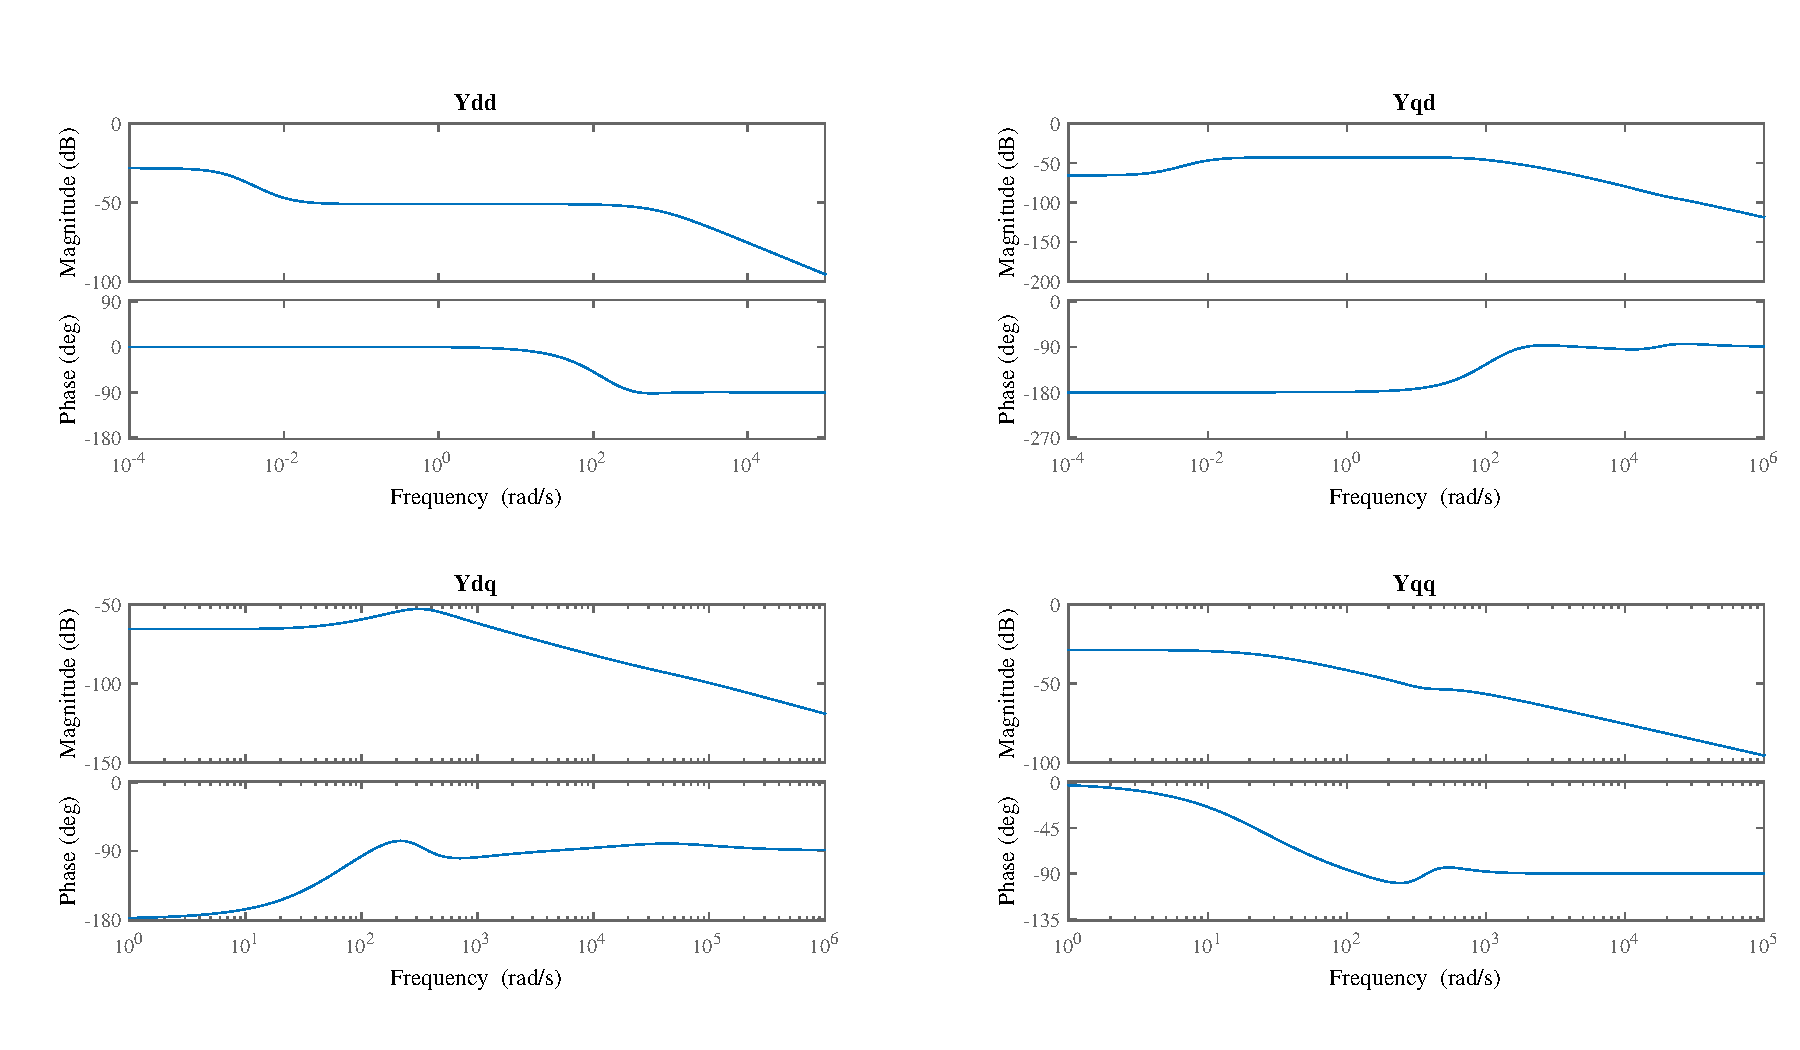
\includegraphics[width=1.2\textwidth]{figures/DroopBode(initial).pdf}
	}
	\caption[Bode diagram of droop inverter]{Bode diagram of droop inverter with optimal parameters}
	\label{res:Droopbode}
\end{figure}


\begin{figure}[ht]
    \centering
     \nonindent
   \makebox[]{
	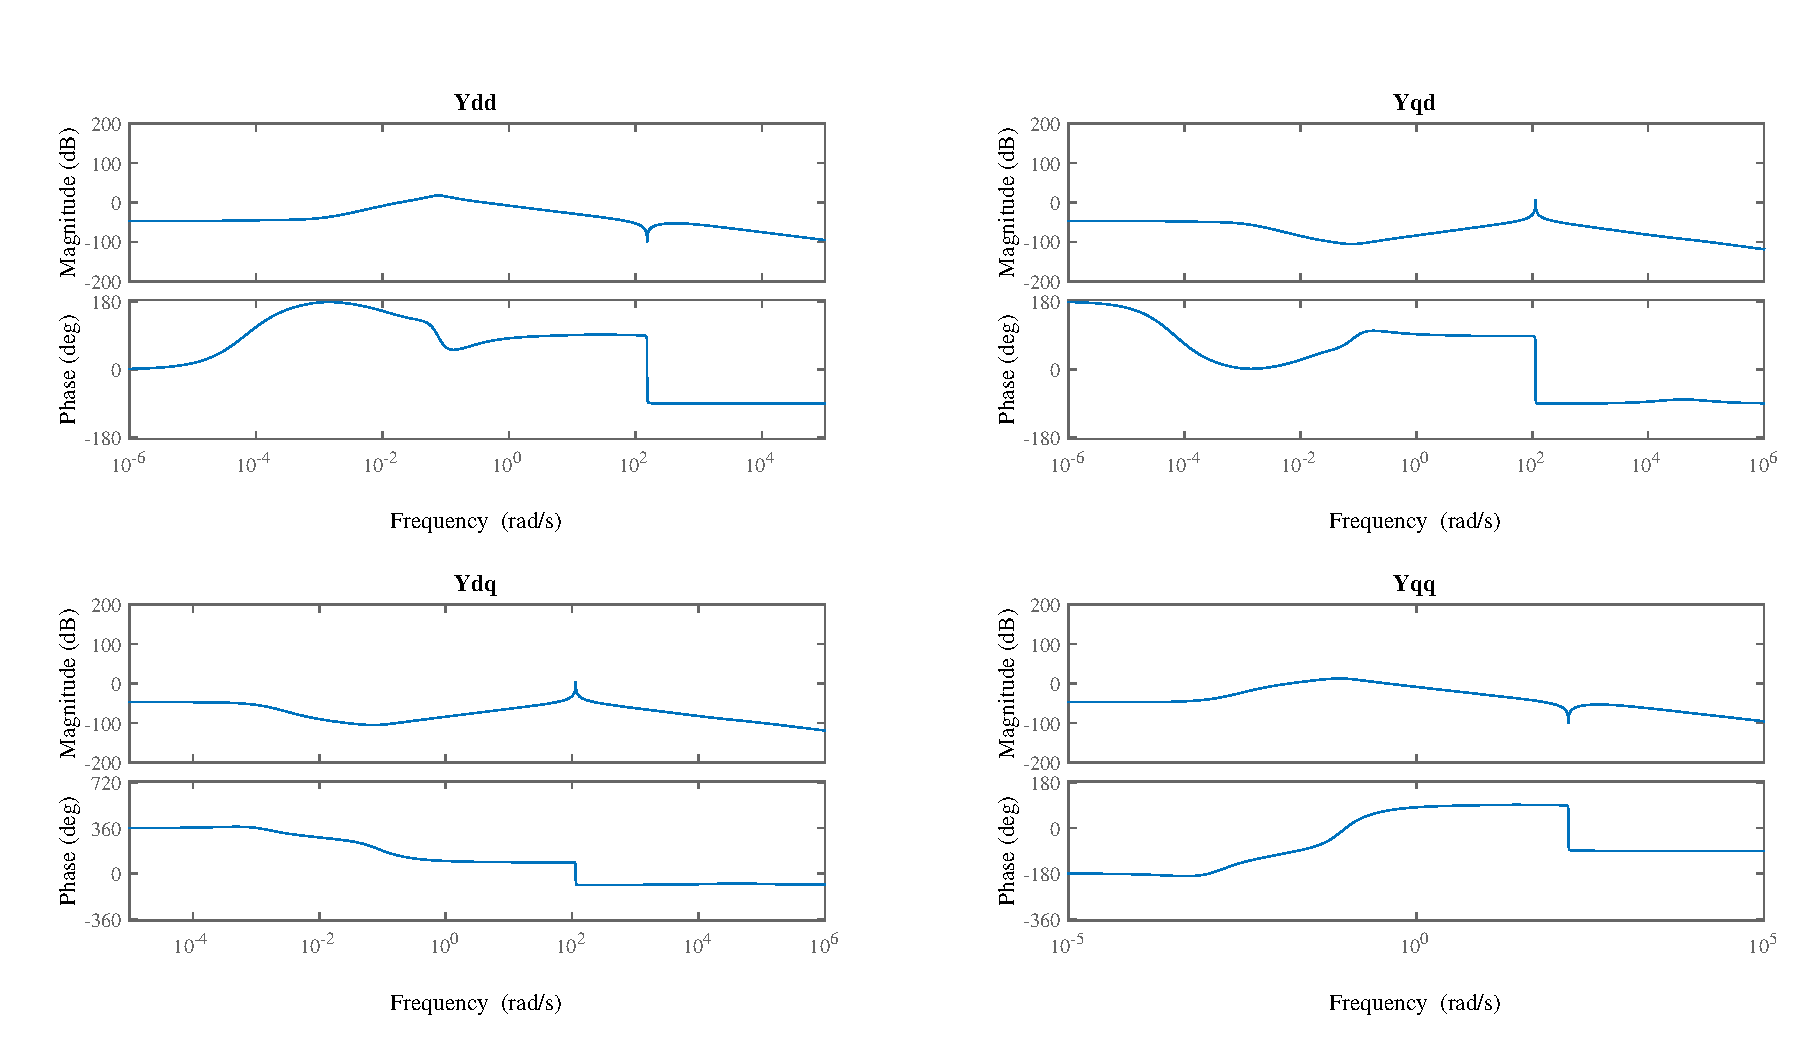
\includegraphics[width=1.2\textwidth]{figures/VILBode(C=0.1).pdf}
	}
	\caption[Bode Diagram of \gls{VIL} inverter]{Bode diagram of \gls{VIL} inverter with optimal parameters}
	\label{res:VILbode}
\end{figure}


\begin{figure}[ht]
    \centering
     \nonindent
   \makebox[]{
	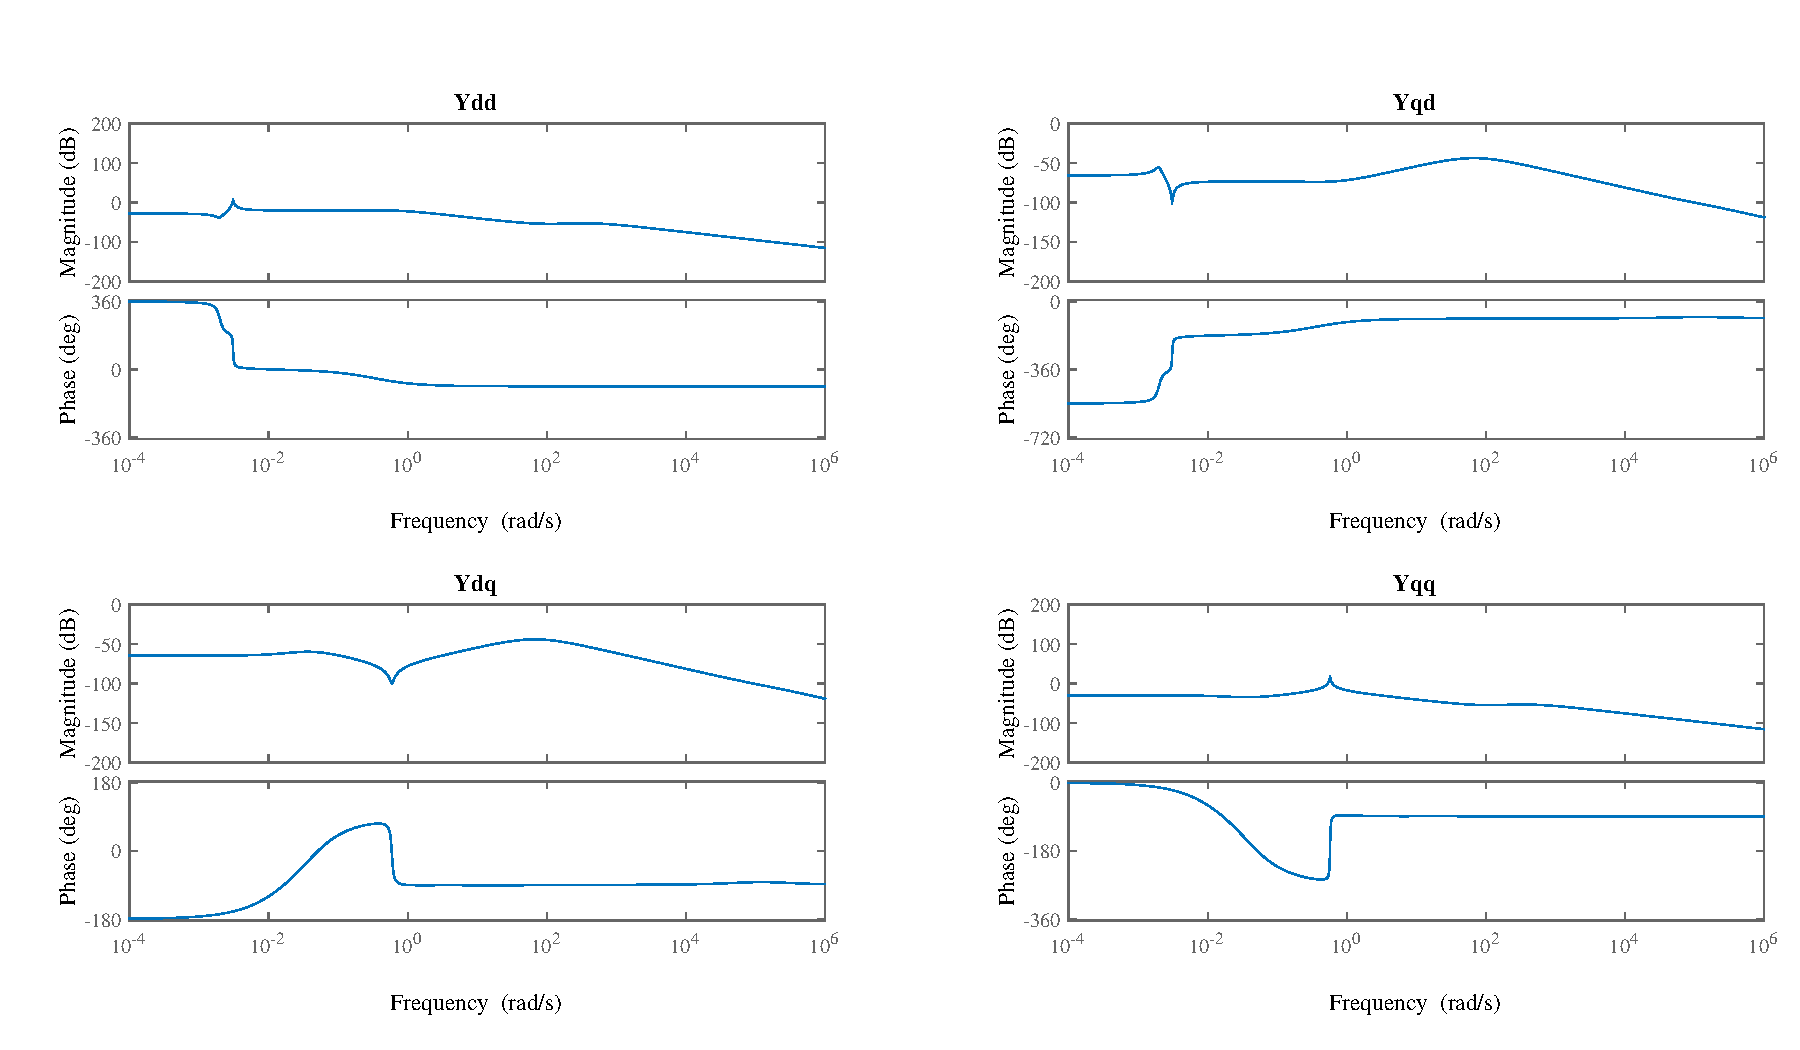
\includegraphics[width=1.2\textwidth]{figures/PSCBode(C=0.1).pdf}
	}
	\caption[Bode diagram of \gls{PSC} inverter]{Bode diagram of \gls{PSC} inverter with optimal parameters}
	\label{res:PSCbode}
\end{figure}


\begin{figure}[ht]
    \centering
     \nonindent
   \makebox[]{
	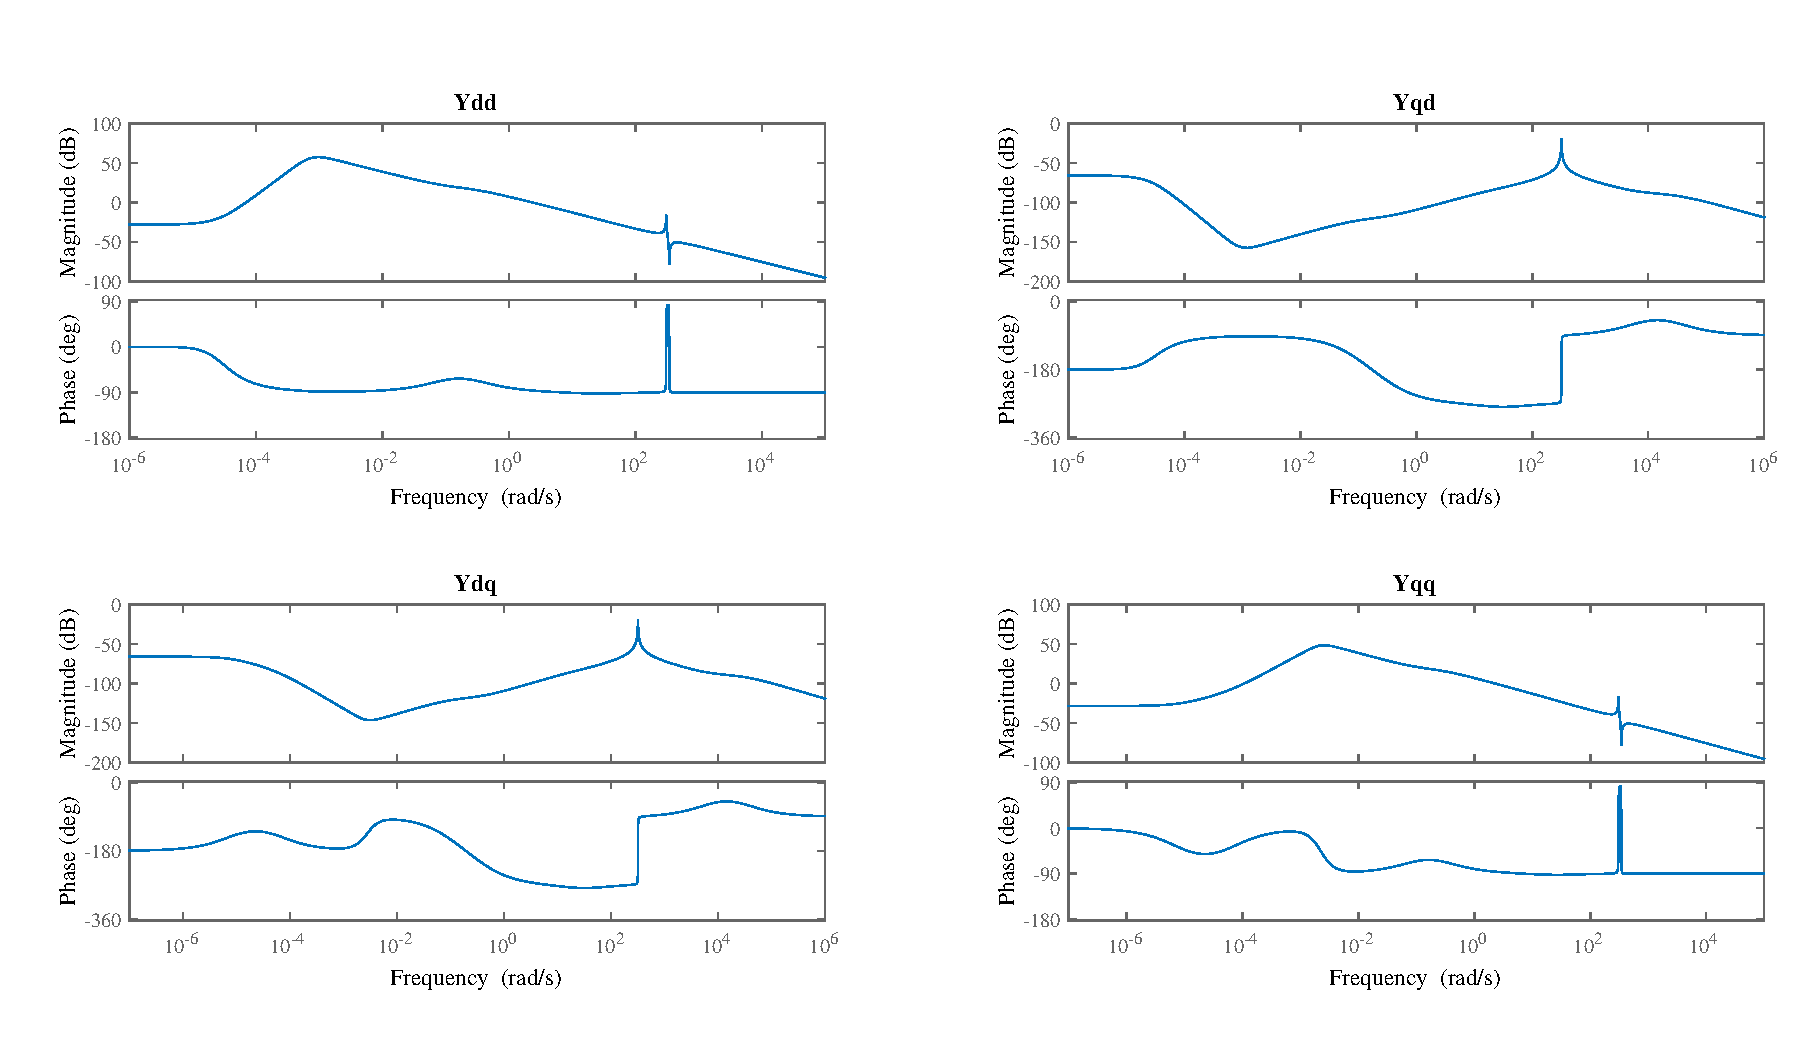
\includegraphics[width=1.2\textwidth]{figures/SynBode(Optimal).pdf}
	}
	\caption[Bode diagram of \gls{Syn} inverter]{Bode diagram of \gls{Syn} inverter with optimal parameters}
	\label{res:Synbode}
\end{figure}

\ref{res:Droopbode} represents the bode response of the Droop \gls{GFM}. The results show that all the gains are negative, meaning that with the optimal parameters, any disturbance with any frequency will have a lower magnitude and be damped. In addition, all $Y_{dd}$, $Y_{qd}$, $Y_{dq}$, and $Y_{qq}$ are acting as a low-pass filter meaning that no high-frequency oscillation will affect the inverter performance.


\ref{res:VILbode} shows the bode diagram of \gls{VIL} inverter. It can be seen that due to the additional term in $\Delta T$ generation, a new pole with the frequency of nearly $10^2$ rad/s is added, which makes the response more complex than the Droop. It also means that for any oscillation in the system, a transient with the frequency of $10^2$ rad/s will circulate in the system. This specific pole will increase the gain in $Y_{qd}$ and $Y_{dd}$ to more than $0$ dB if an oscillation near $10^2$ (rad/s) happens.


\ref{res:PSCbode} shows the bode results the \gls{PSC} inverter. The results show a stable behavior in $Ydq$ and $Yqd$. However, in the vicinity of a specific pole, the magnitude becomes more than $0 (dB)$. Another Noteworthy point is that all four transfer functions of PSC can be modeled as a low-pass filter like the droop controller.


\ref{res:Synbode} shows the bode results the \gls{Syn} inverter. According to the \ref{res:Synbode} \gls{syn} Inverter has the most complex bode diagram among GFMs. The most highlightable behavior of the \gls{Syn} inverter is the very sharp magnitude and angle change in a certain frequency range. This bode diagram will ensure oscillatory behavior in any disturbance. Like the \gfl{PSC}, the $Ydq$ and $Yqd$ can decrease any disturbance.

\begin{figure}[ht]
    \centering
     \nonindent
   \makebox[]{
	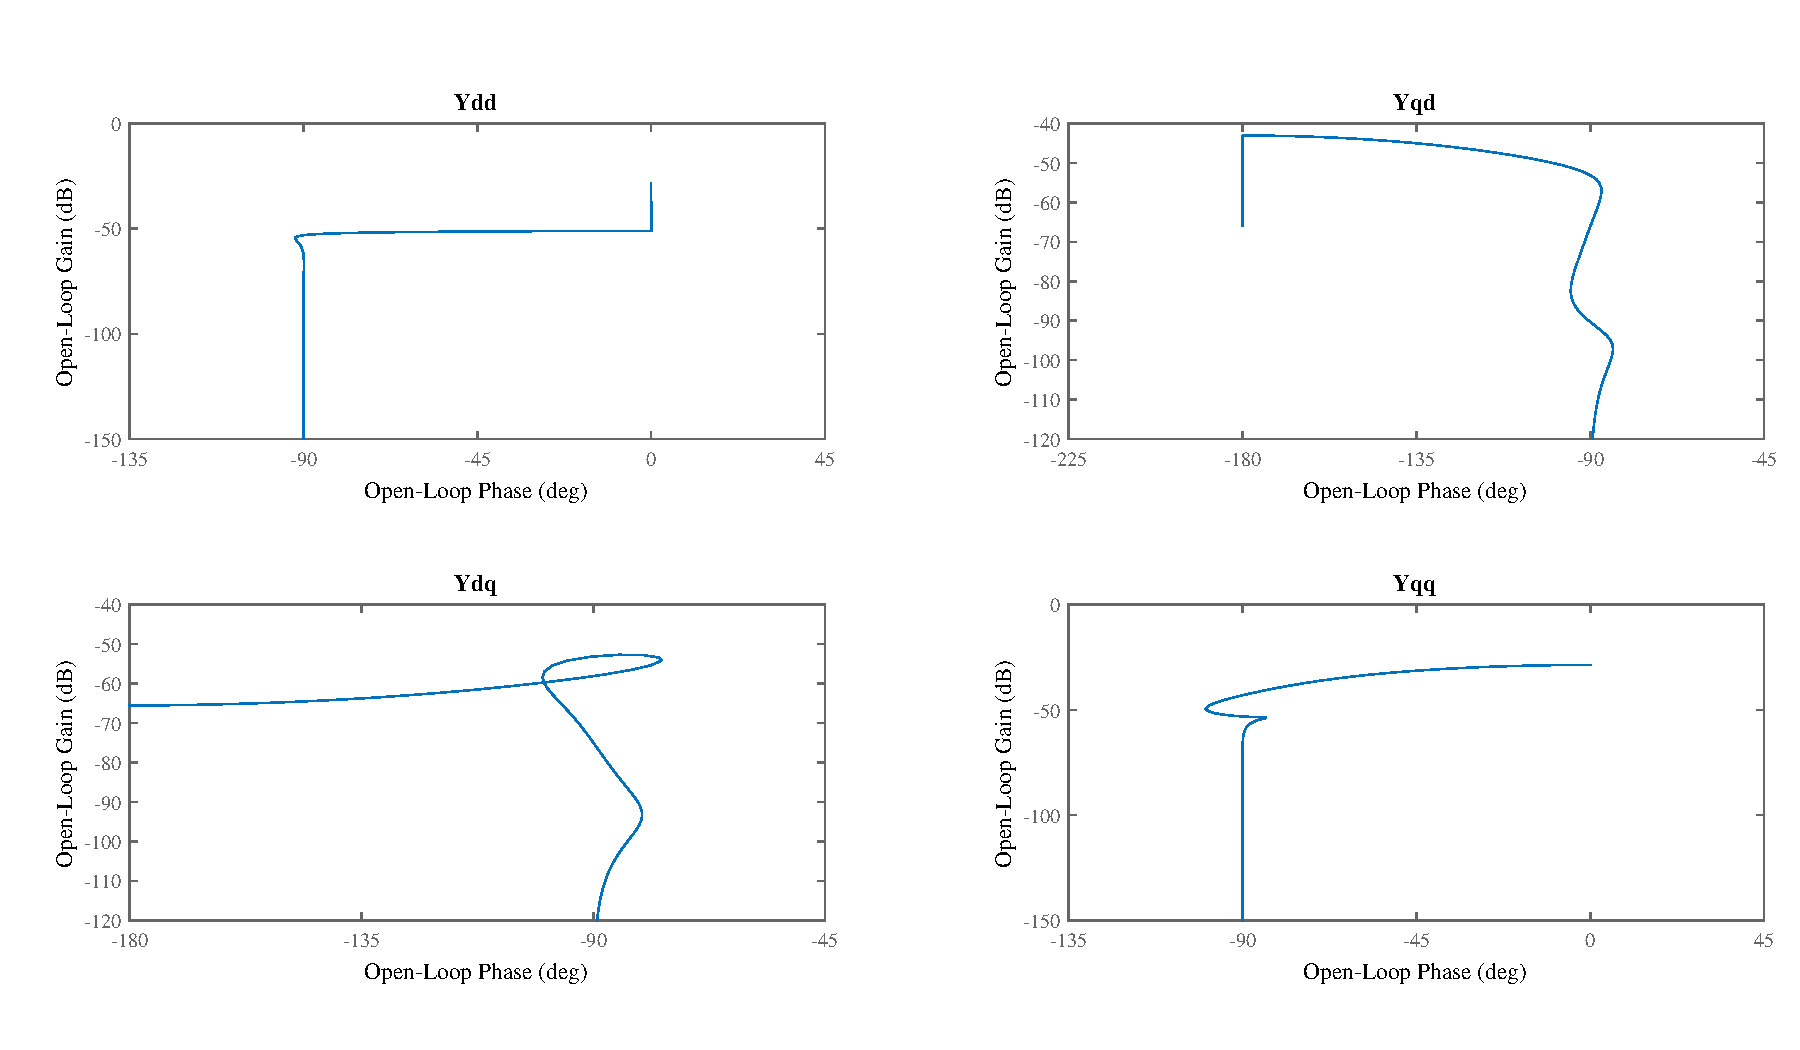
\includegraphics[width=1.2\textwidth]{figures/DroopNichols(initial).pdf}
	}
	\caption[Nichols diagram of Droop GFM  inverter]{Nichols diagram of Droop GFM  inverter for optimal parameters}
	\label{res:DroopNichols}
\end{figure}

\begin{figure}[ht]
    \centering
     \nonindent
   \makebox[]{
	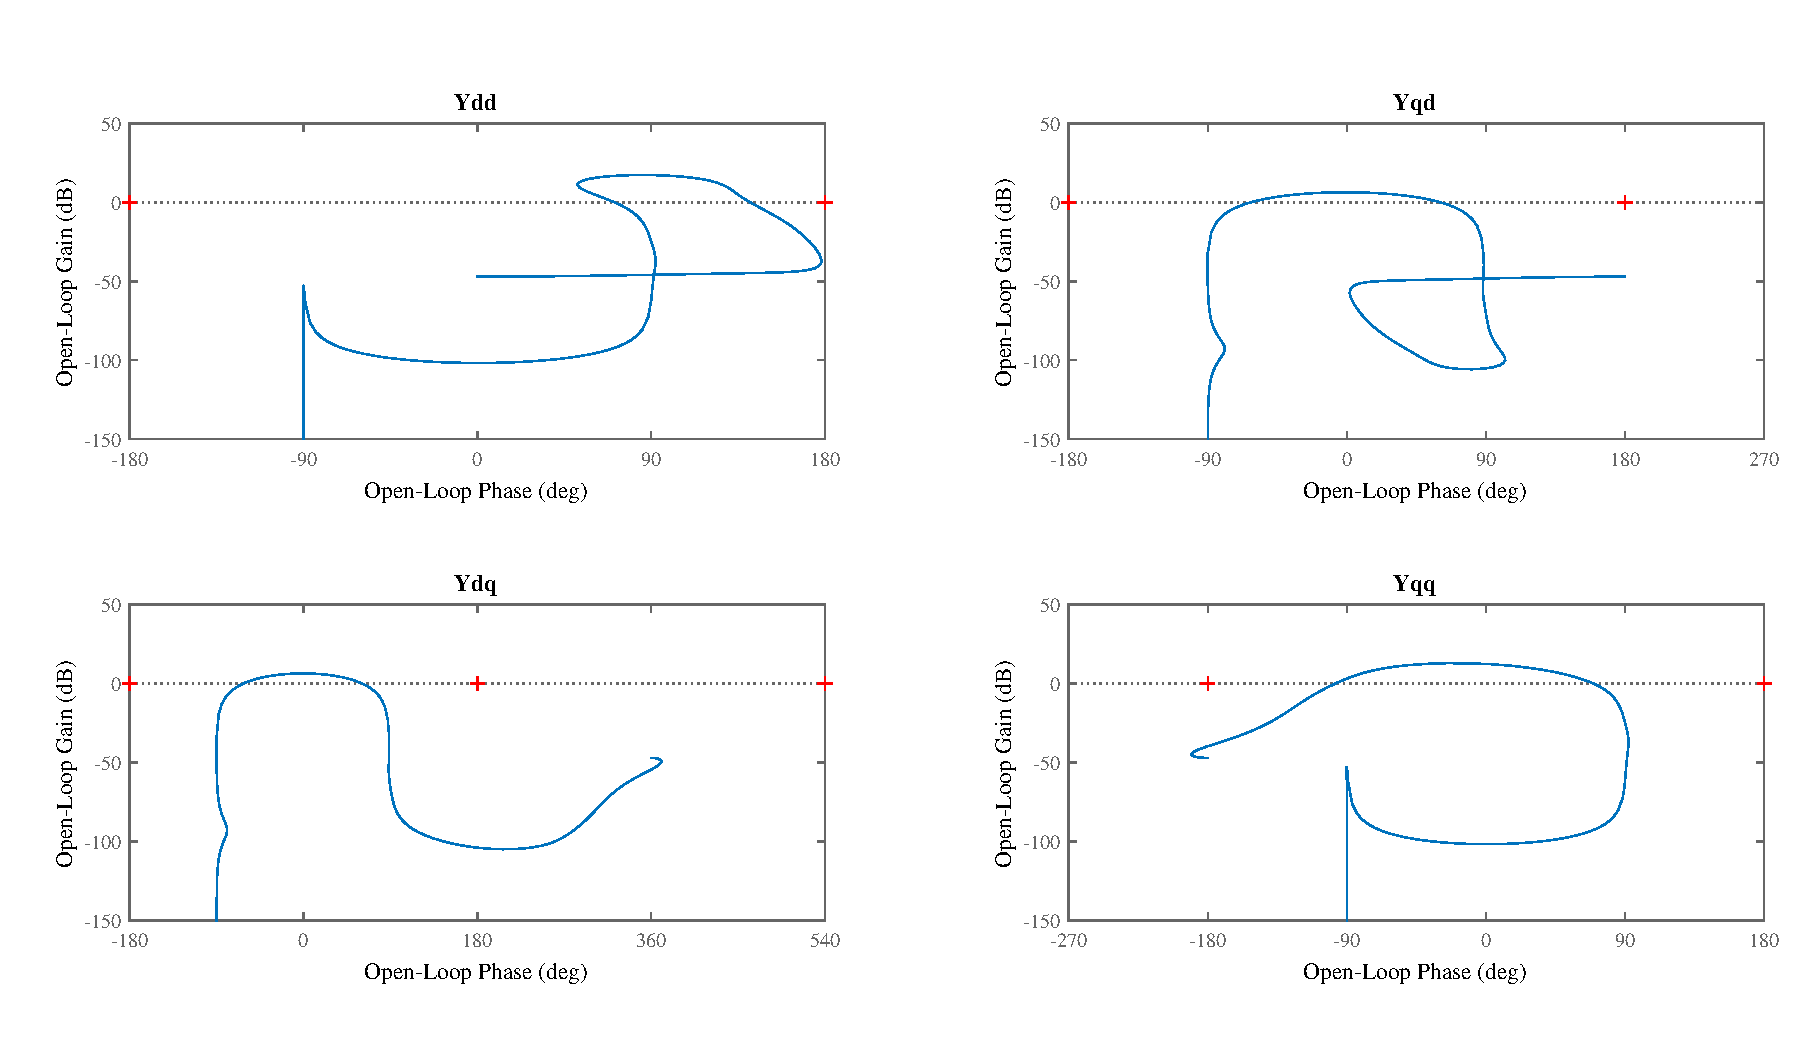
\includegraphics[width=1.2\textwidth]{figures/VILNichols(C=0.1).pdf}
	}
	\caption[Nichols diagram of \gls{VIL} inverter]{Nichols diagram of \gls{VIL} inverter for optimal parameters}
	\label{res:VILNichols}
\end{figure}

\begin{figure}[ht]
    \centering
     \nonindent
   \makebox[]{
	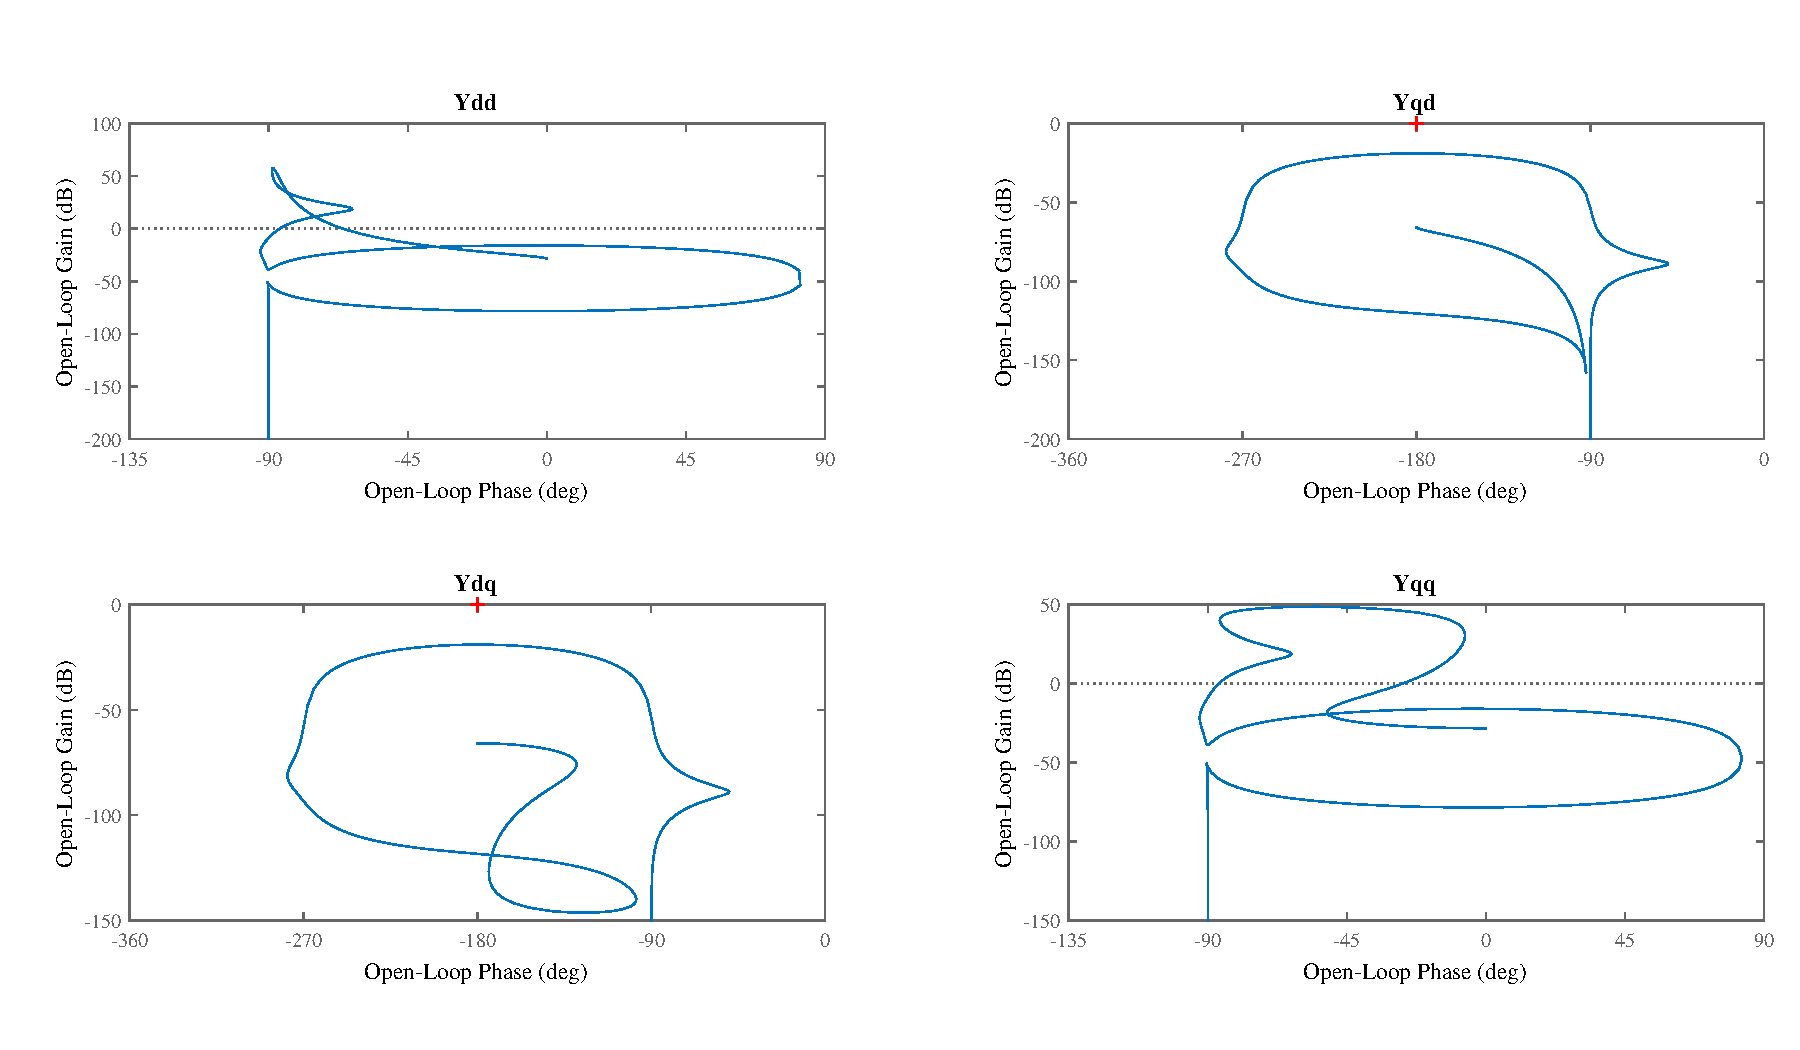
\includegraphics[width=1.2\textwidth]{figures/SYNNichols(Optimal).pdf}
	}
	\caption[Nichols diagram of of \gls{Syn} inverter]{Nichols diagram of \gls{Syn} inverter for optimal parameters}
	\label{res:SynNichols}
\end{figure}

\begin{figure}[ht]
    \centering
     \nonindent
   \makebox[]{
	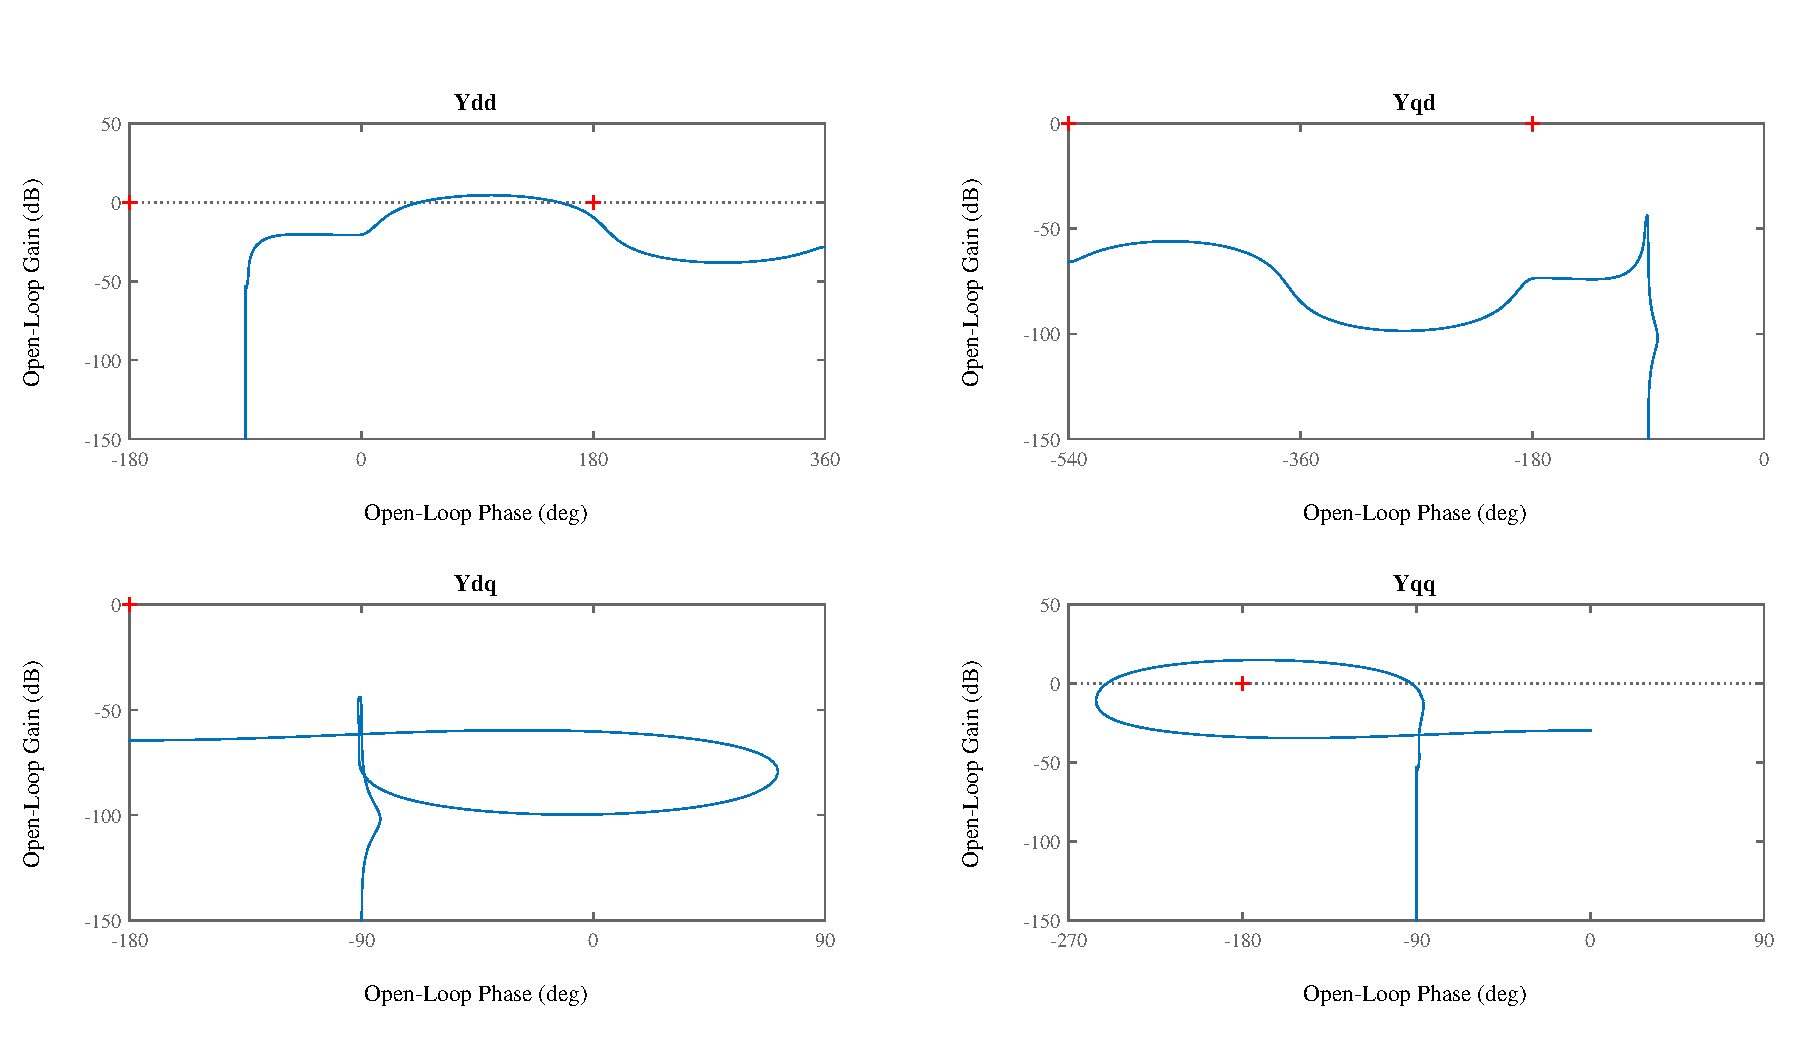
\includegraphics[width=1.2\textwidth]{figures/PSCNichols(C=0.1).pdf}
	}
	\caption[Nichols diagram of \gls{PSC} inverter]{Nichols diagram of \gls{PSC} inverter for optimal parameters}
	\label{res:PSCNichols}
\end{figure}
 In this subsection, Nichols diagram of all GFM converters is presented. Nichols diagram is a frequency domain indicator for the transfer function. Nichols can be used for model reduction. The model reduction is necessary for dealing with multiple inverters. Nichols plots the admittance of each component with the gain and phase in the axes. The results show that the Droop GFM has the most straightforward Nichols diagram with two major sharp points in $Ydd$ and four major sharp points in $Ydq$ whereas the \gls{Syn} inverter has the most complex Nichols diagram. Therefore, the Droop strategy is the easiest to make the model reduction study. Another noteworthy point is that the four transfer matrices may have very different behaviors in a specific inverter. This makes the parameter tuning very complex because all four transfer functions must be maintained in the stable margin simultaneously.
 
 All four transfer functions have a negative gain with varying frequency for the Droop inverter. Especially in $Y_{dd}$ with the change of frequency, the open-loop phase jumps from zero to $-90^o$; however, In \gls{VIL} with the same parameters, all four transfer functions that have a gain of more than 0 dB. In addition, in $Y_{dq}$, the open-loop phase varies between $360^o$ and $-90$, which is not very well behaved. The Nichols diagram of \gls{Syn} inverter, which is shown in \ref{res:SynNichols} is the most complex among other inverters. Although the results for $Y_{dq}$ and $Y_{qd}$ are both in the stable range, the $Y_{dq}$ and $Y_{qd}$ appear to behave very arbitrary and also in some points they get a positive gain in perturbation. \gls{PSC} control results are shown in \ref{res:PSCNichols}. The behavior of the \gls{PSC} is more similar to Droop with a not very complex behavior.
 
\section{Parameter Sensitivity Analysis of \gls{GFL}}


\begin{table}[ht]
\centering
\caption[Optimal GFL Parameters]{Optimal GFL Parameters}
\label{res:param}
\resizebox{.8\textwidth}{!}{%
\begin{tabular}{llllll}
\hline
Parameter & Value & Parameter & Value & Parameter & Value  \\ \hline
L_1 & 0.6 & t_{del} & $1/40000$ & K_p_C & 10   \\

L_2 & 0.6 & 17 & 16 & K_I_C & 0.1 \\

C & 0.5 & K_p_Q  & 100 & K_p_P  & 100\\

D & 1 & K_I_Q  & 10 & K_I_P  & 10 \\

K_p_{PLL}  & 100 & K_I_{PLL}  & 6400 & $\omega_c$ & 10000\\
\hline
\end{tabular}
}
\end{table}

\begin{figure}[ht]
\begin{center}
    \centering
   \nonindent
   \makebox[]{
	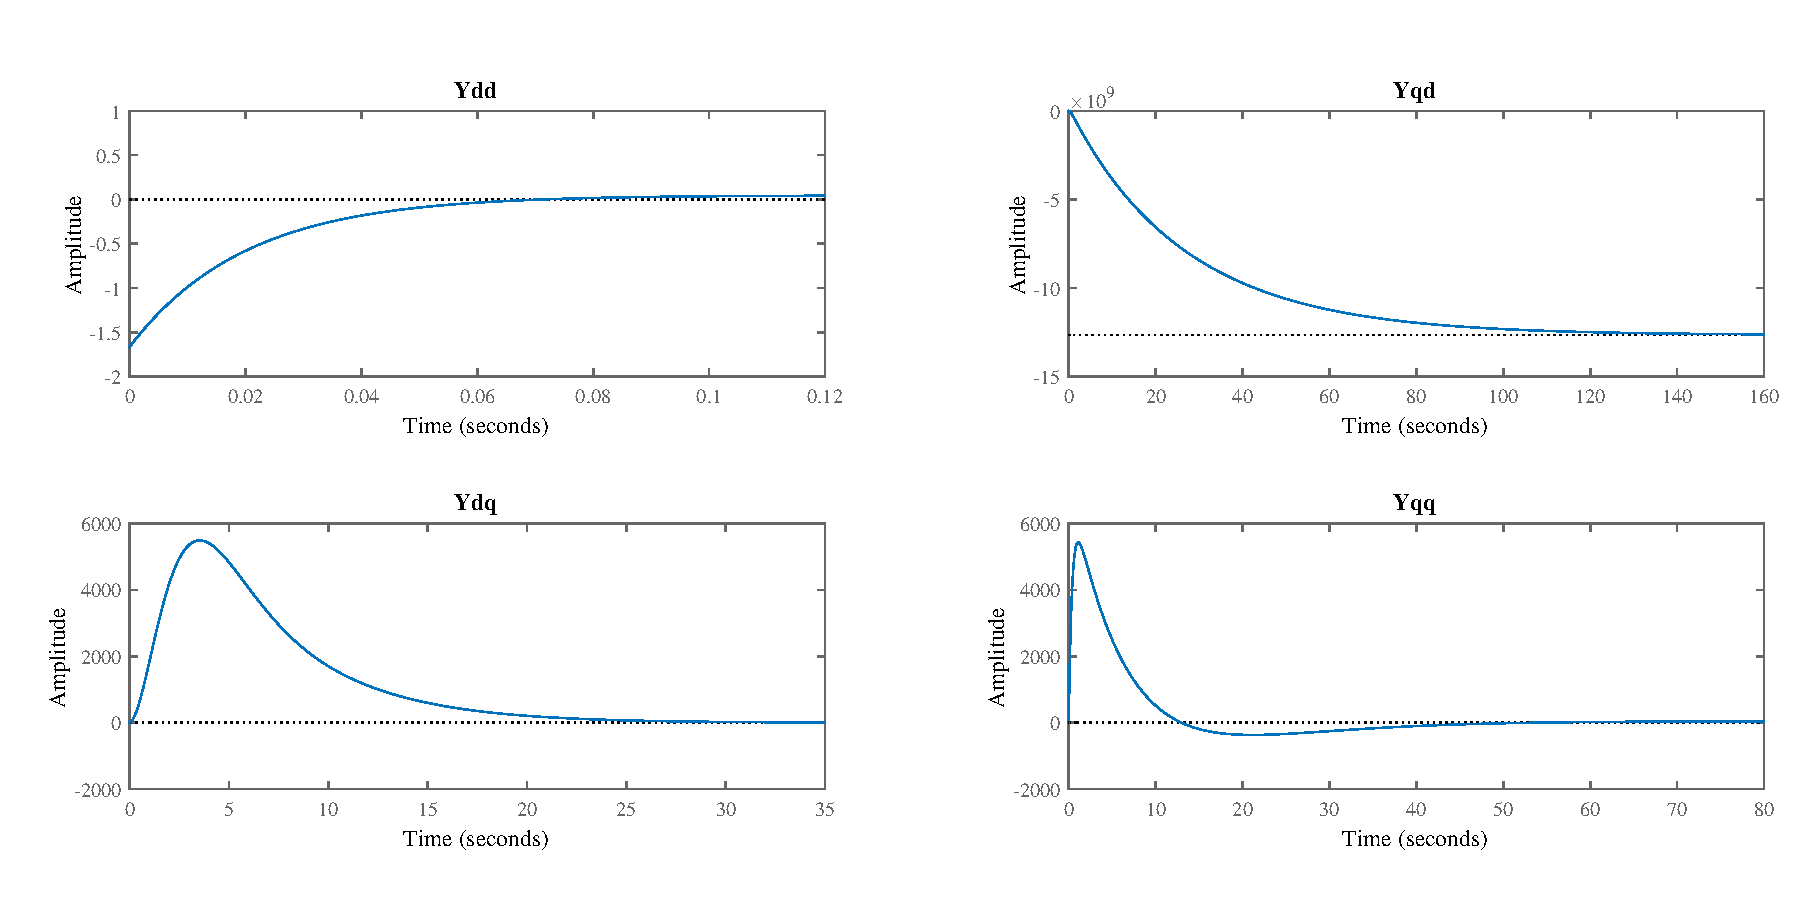
\includegraphics[width=1.2\textwidth]{figures/Base.pdf}}
	\caption[Basic impulse response ]{Basic impulse response for tuned parameters of \gls{GFL}.}
	\label{res:base}
	\end{center}
\end{figure}
In this part of the results, sensitivity analysis is performed for the parameters mentioned in \ref{parameters} for the \gls{GFL}. The Base stable impulse response of the \gls{GFL} inverter is highlighted in \ref{res:base} and the corresponding parameters are mentioned in \ref{res:param}

As it can be seen in \ref{res:base}, all four transfer functions result in a stable behavior, and all of the magnitudes are damped after a particular time. However, in order to better understand the effect of each important parameter in impulse behavior, sensitivity analyses are performed by repetition of simulations for different parameters. 

\subsection{steady-state Angle}



\begin{figure}[ht]
\begin{center}
    \centering
   \nonindent
   \makebox[]{
	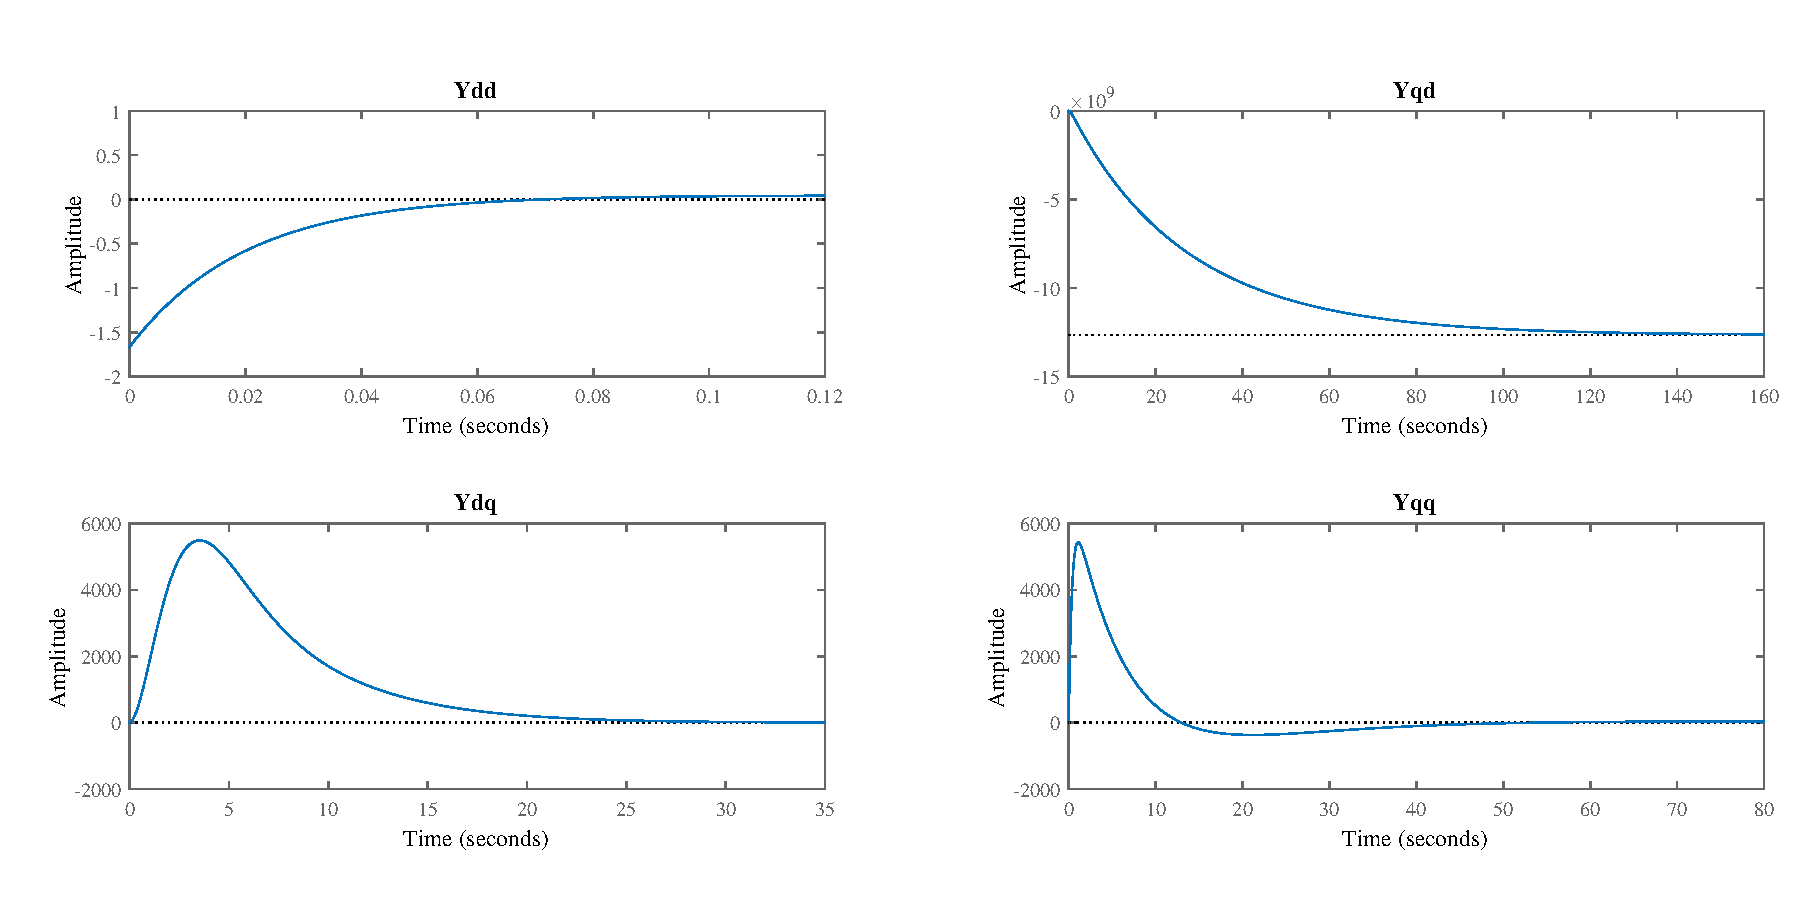
\includegraphics[width=1.2\textwidth]{figures/Base.pdf}}
	\caption[GFL impulse response for $\theta=0$]{GFL impulse response for $\theta=0$.}
	\label{res:theta0}
	\end{center}
\end{figure}
\begin{figure}[ht]
\begin{center}
    \centering
   \nonindent
   \makebox[]{
	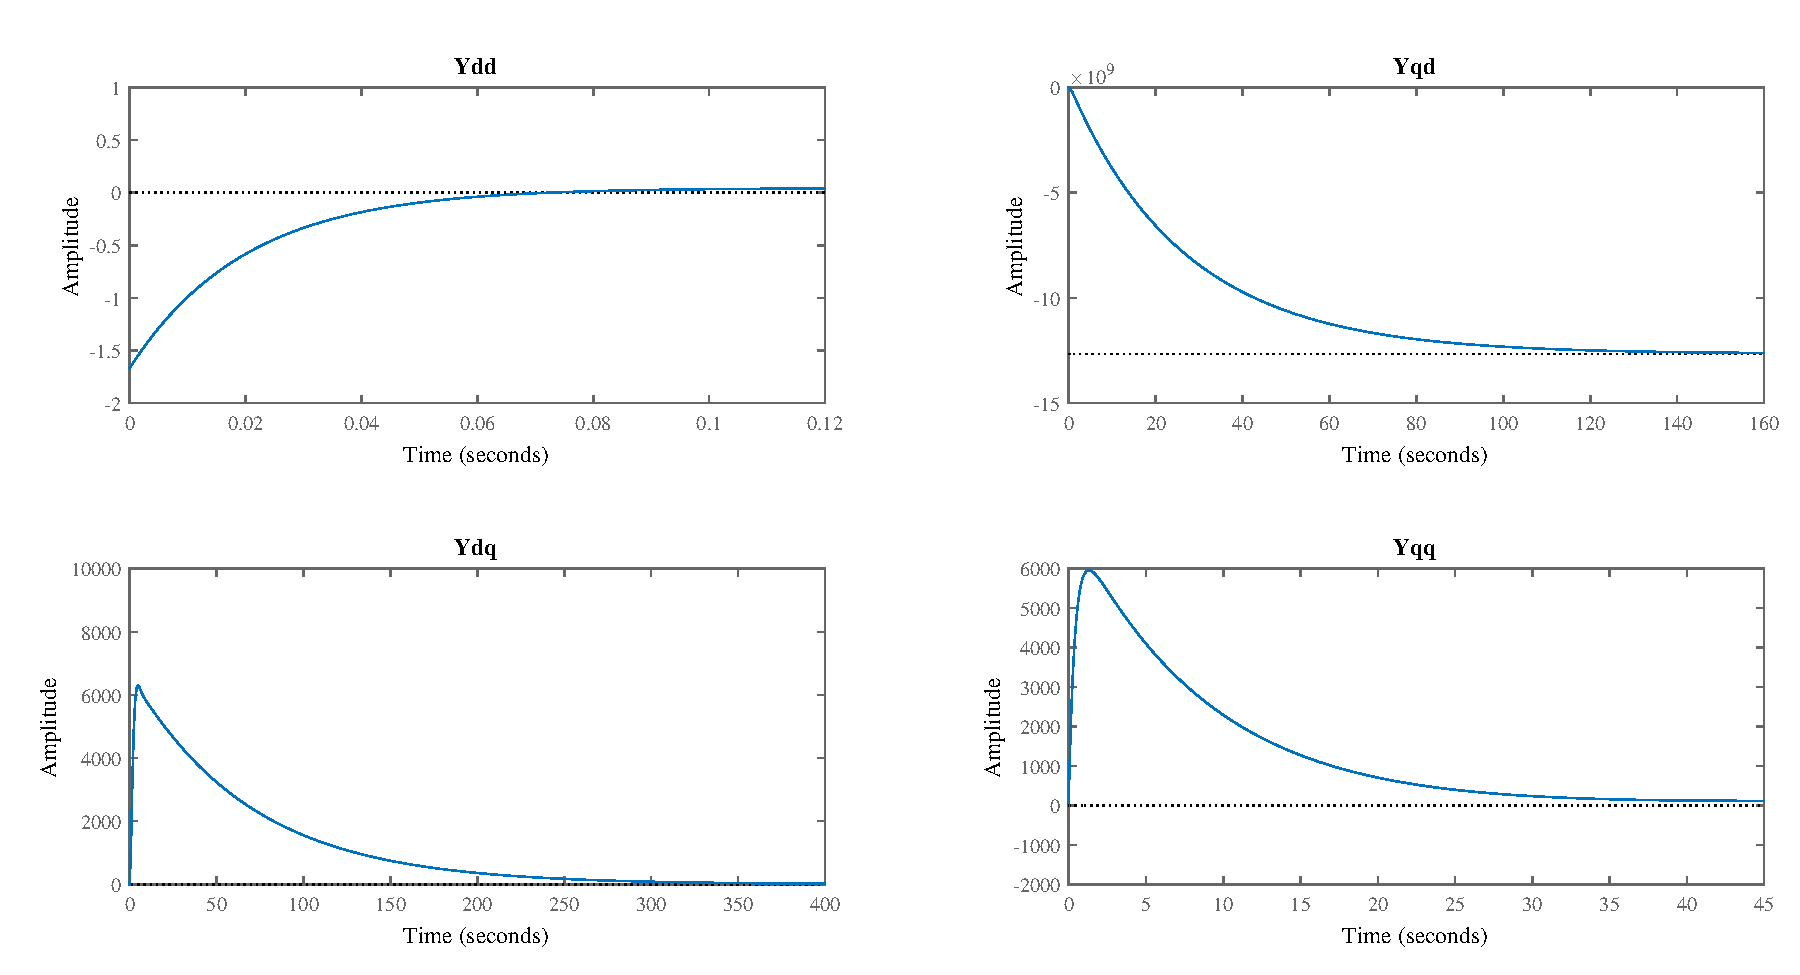
\includegraphics[width=1.2\textwidth]{figures/Teta(0.004).pdf}}
	\caption[GFL impulse response for $\theta=0.004$]{GFL impulse response for $\theta=0.004$.}
	\label{res:theta0.004}
	\end{center}
\end{figure}


\begin{figure}[ht]
\begin{center}
    \centering
   \nonindent
   \makebox[]{
	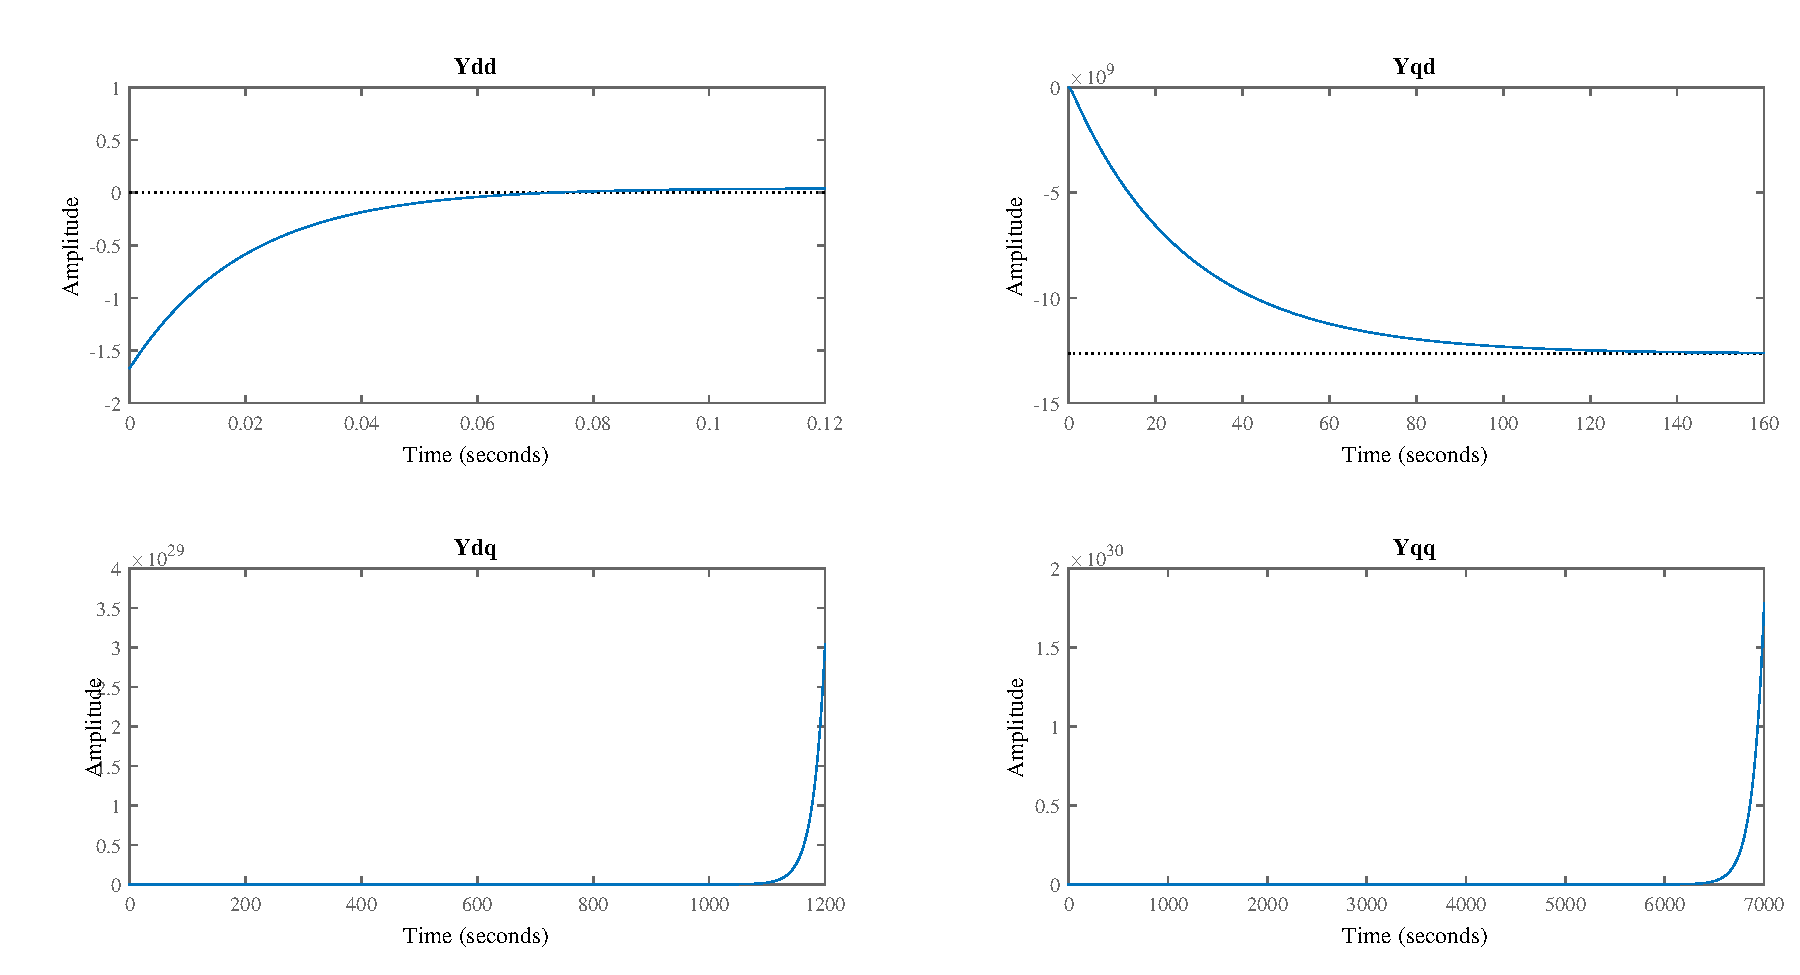
\includegraphics[width=1.2\textwidth]{figures/Teta(0.006).pdf}}
	\caption[GFL impulse response for $\theta=0.006$]{GFL impulse response for $\theta=0.006$.}
	\label{res:theta0.006}
	\end{center}
\end{figure}

\begin{figure}[ht]
\begin{center}
    \centering
   \nonindent
   \makebox[]{
	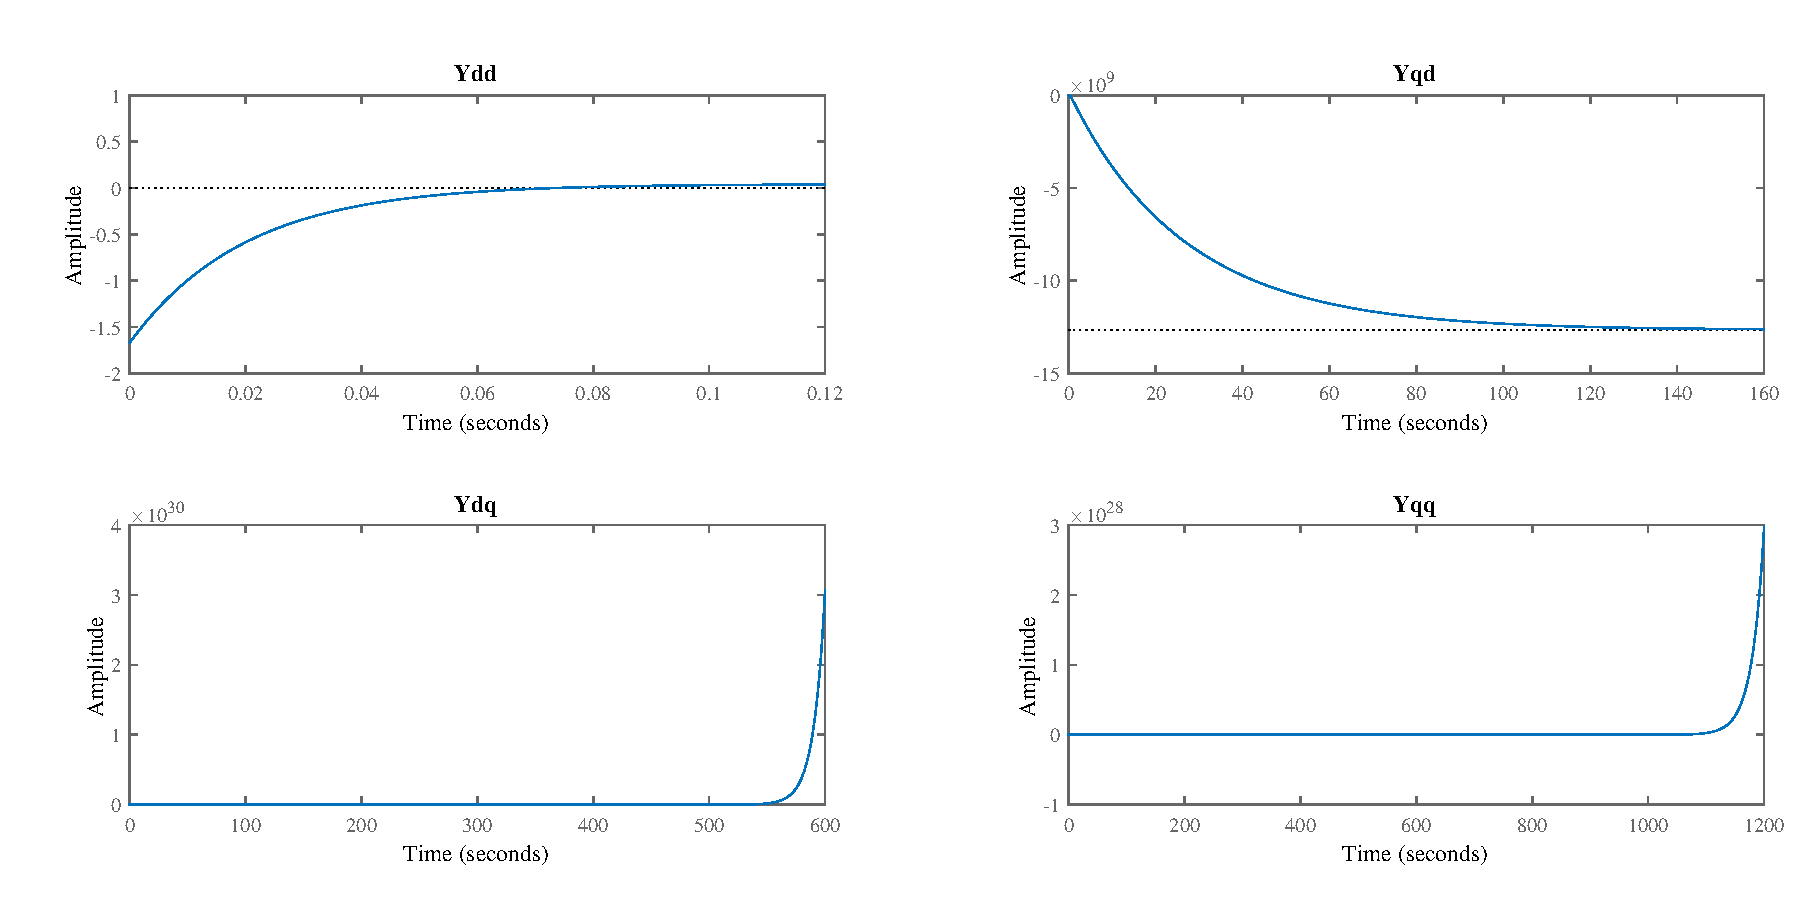
\includegraphics[width=1.2\textwidth]{figures/Teta(0.008).pdf}}
	\caption[GFL impulse response for $\theta=0.008$]{GFL impulse response for $\theta=0.008$.}
	\label{res:theta0.008}
	\end{center}
\end{figure}
The steady-state angle is the difference between local and global $dq$ frames. In power systems, the operation angles of generators may be different. Therefore this difference must be included in inter-area oscillations. The results of changing the steady-state angle from $0$ rad to $0.006$ rad are presented in \cref{res:theta0,res:theta0.004,res:theta0.006,res:theta0.008}.

Evaluating \cref{res:theta0,res:theta0.004,res:theta0.006,res:theta0.008} clears that there is a certain margin for $\theta$ that  increasing the amount of $\theta$ more than that margin deteriorates the small signal stability, since the impulse response of $Y_{qd}$ and $Y_{qq}$ are converging to infinite amount. This shows that a few poles exist on the right side of the real axis, which drives the small signal stability of the inverter to an unstable margin. The margin of $\theta$, in this case, is around 0.005 rad. The results are analogous to synchronous generators where the internal angle must be in a certain range generator to remain stable.

\subsection{Current Control Block}

\begin{figure}[ht]
\begin{center}
    \centering
   \nonindent
   \makebox[]{
	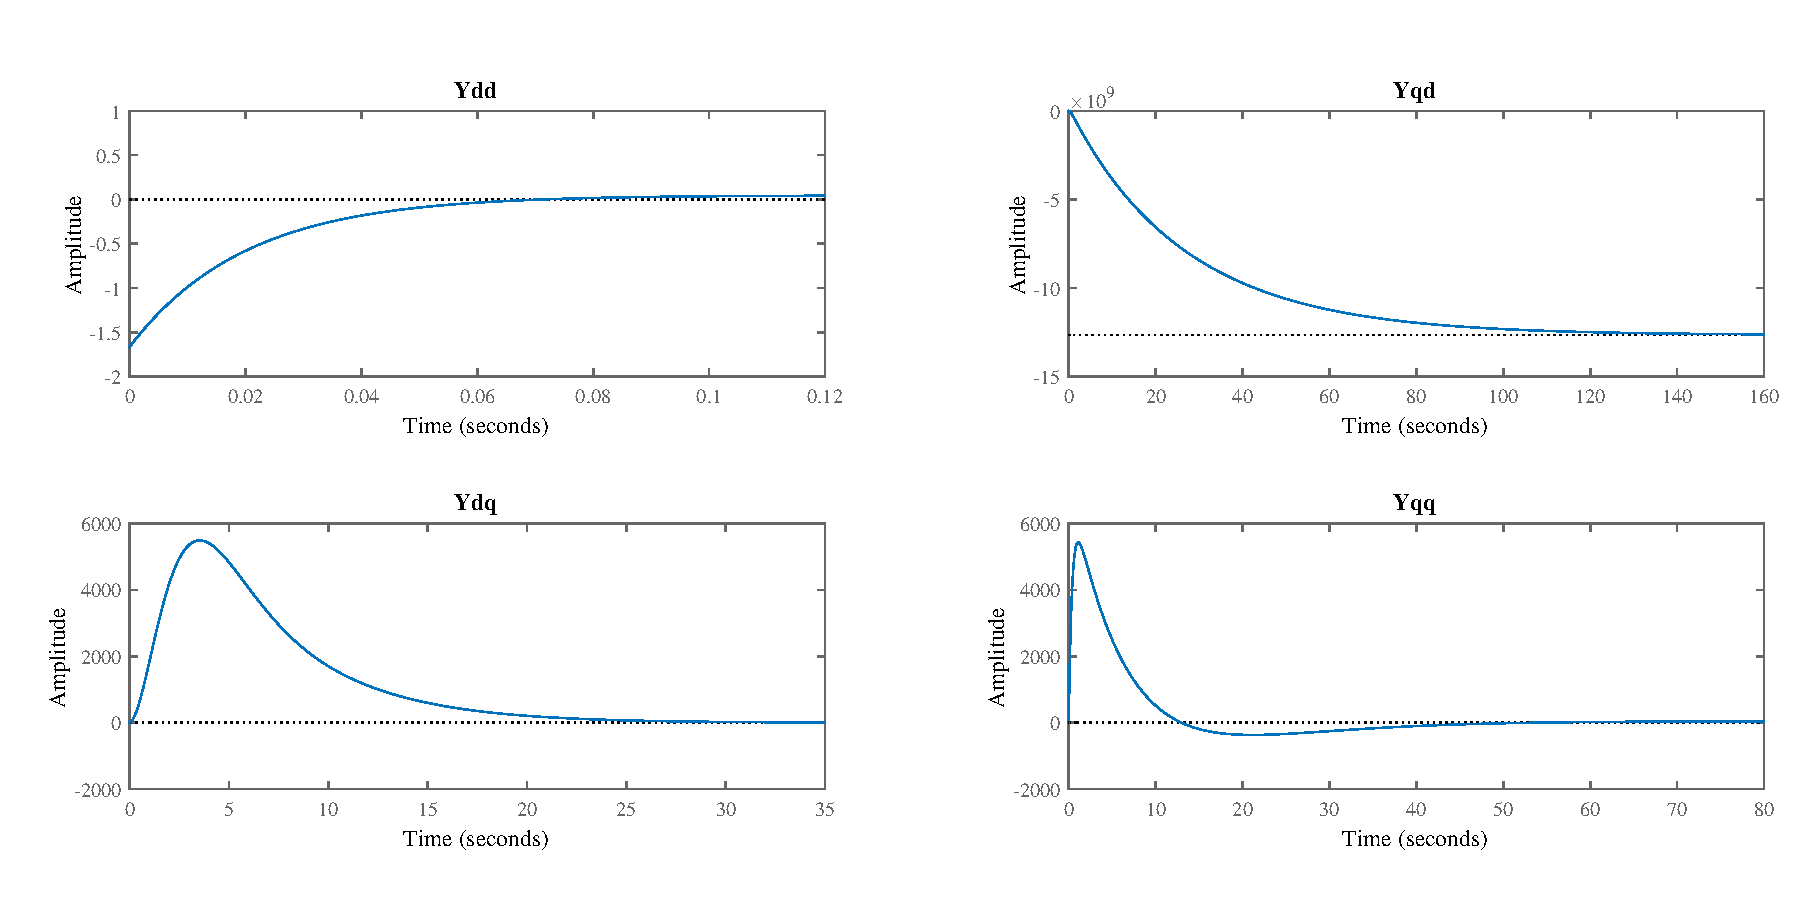
\includegraphics[width=1.2\textwidth]{figures/Base.pdf}}
	\caption[GFL impulse response for $K_{PC}=100$]{GFL impulse response for $K_{PC}=100$.}
	\label{res:Kpc(100)}
	\end{center}
\end{figure}

\begin{figure}[ht]
\begin{center}
    \centering
   \nonindent
   \makebox[]{
	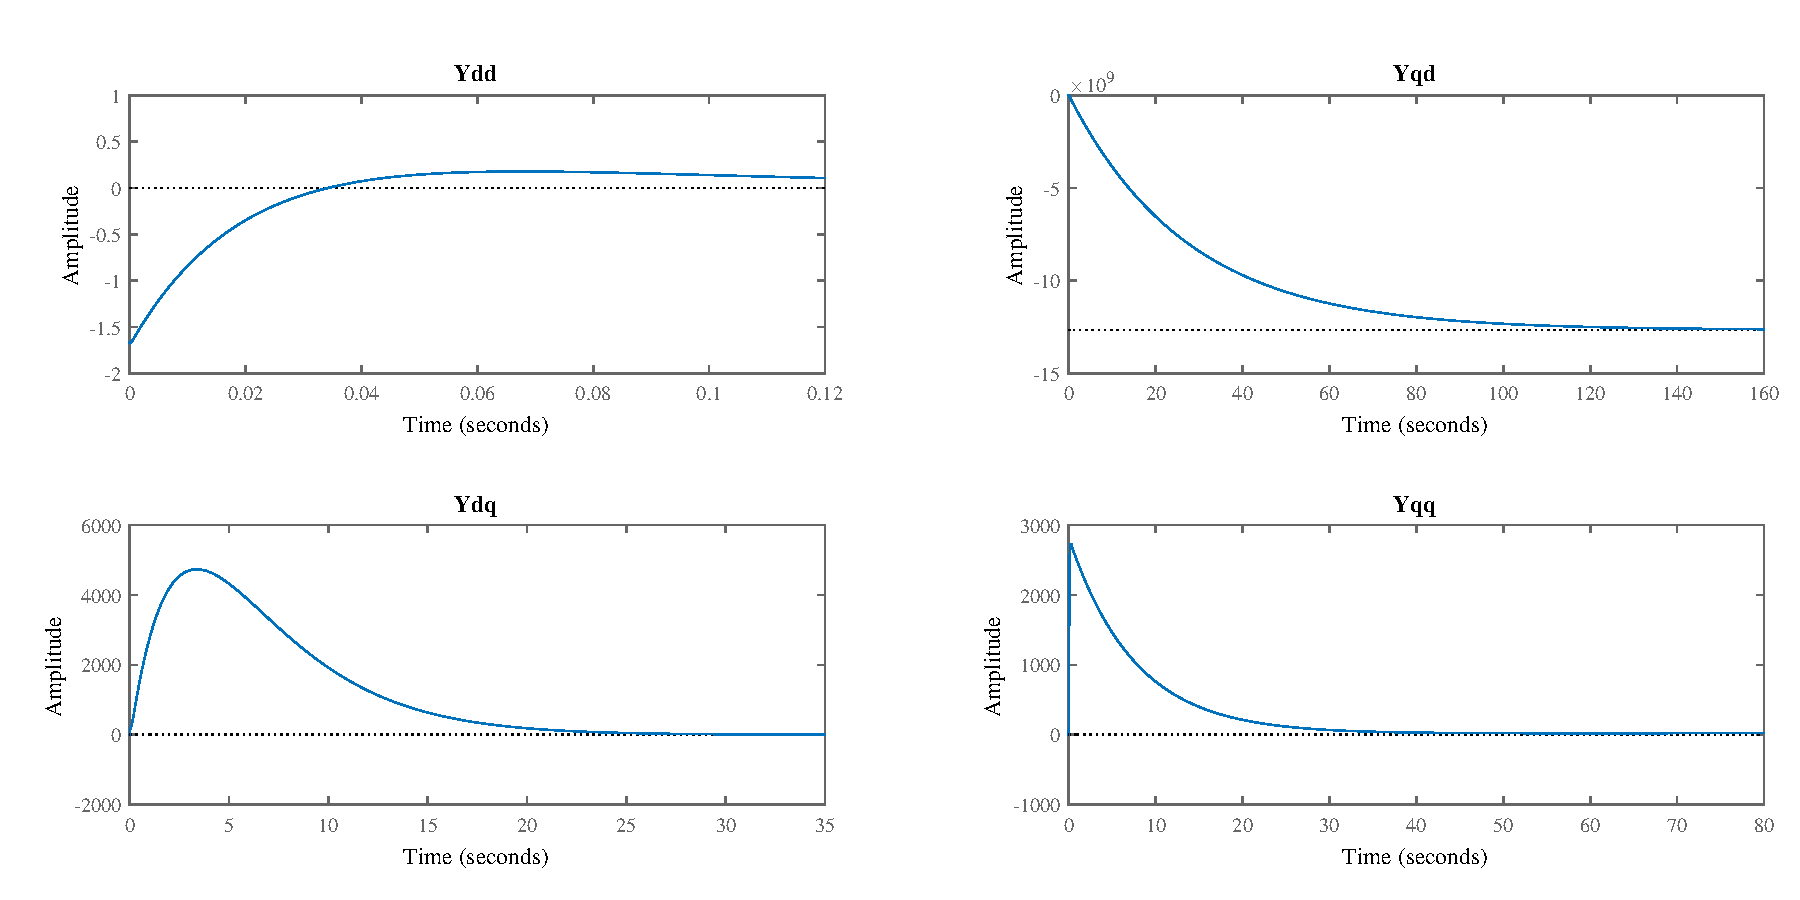
\includegraphics[width=1.2\textwidth]{figures/Kpc(10).pdf}}
	\caption[GFL impulse response for $K_{PC}=10$]{GFL impulse response for $K_{PC}=10$.}
	\label{res:Kpc(10)}
	\end{center}
\end{figure}


\begin{figure}[ht]
\begin{center}
    \centering
   \nonindent
   \makebox[]{
	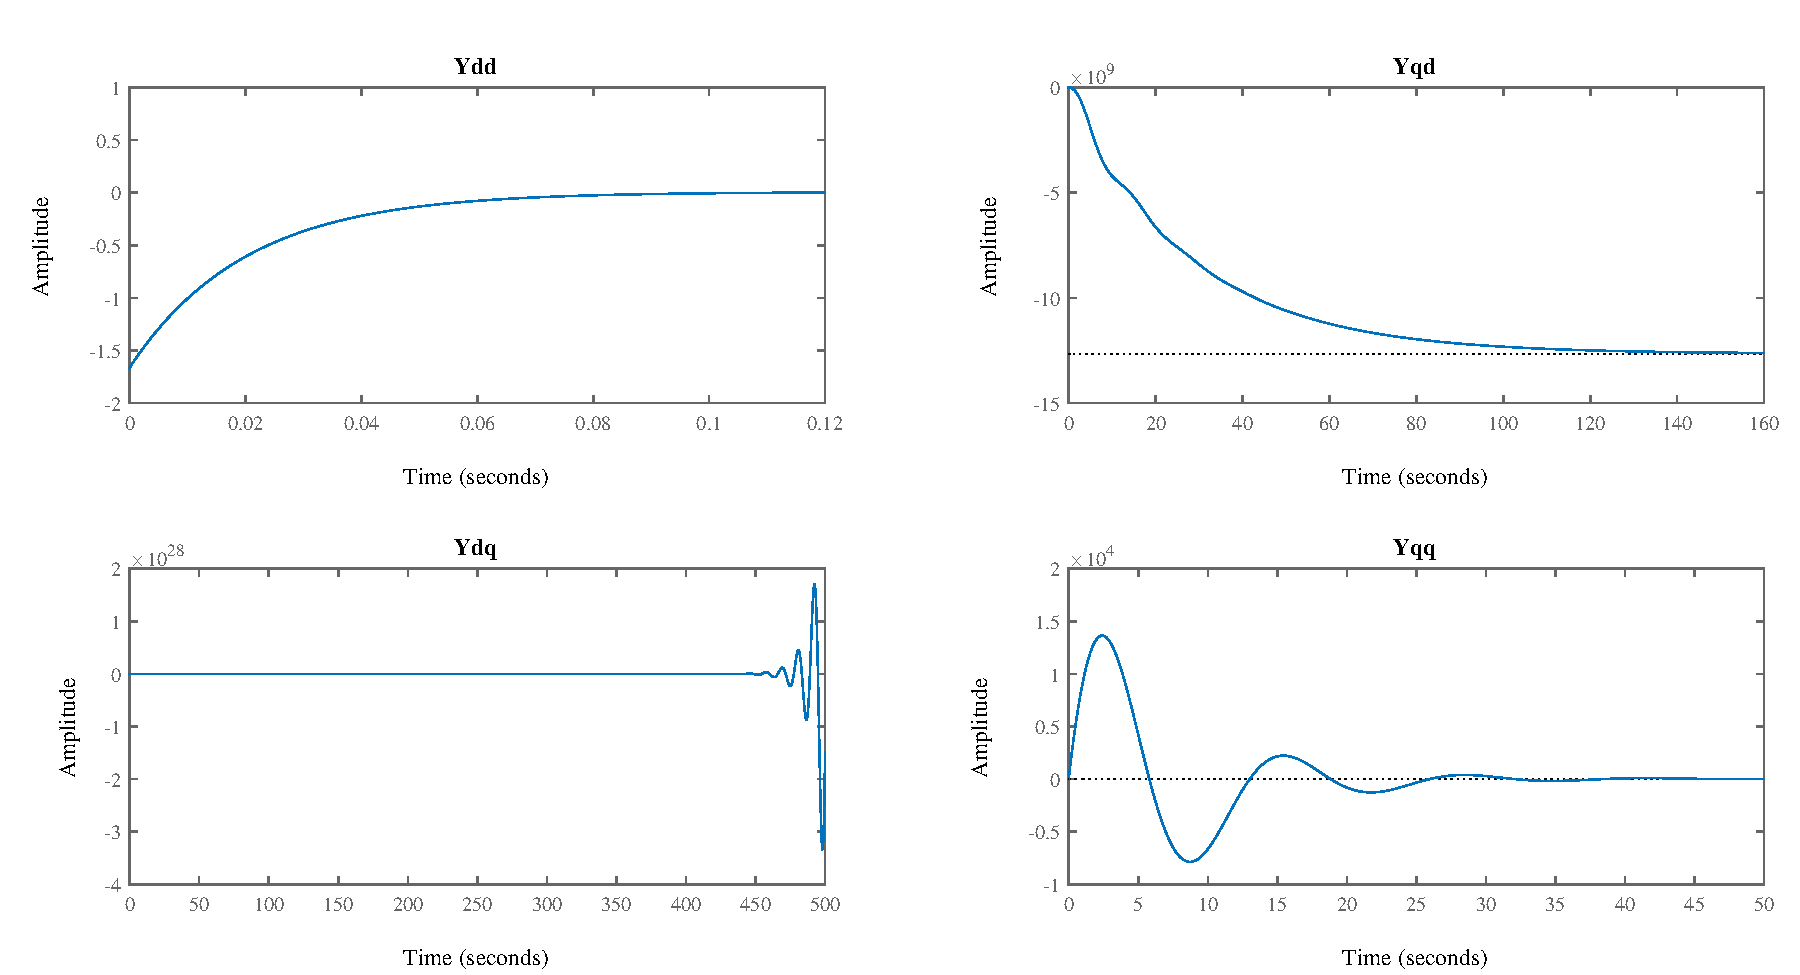
\includegraphics[width=1.2\textwidth]{figures/Kpc(0.1).pdf}}
	\caption[GFL impulse response for $K_{PC}=0.1$]{GFL impulse response for $K_{PC}=0.1$.}
	\label{res:Kpc(0.1)}
	\end{center}
\end{figure}


\begin{figure}[ht]
\begin{center}
    \centering
   \nonindent
   \makebox[]{
	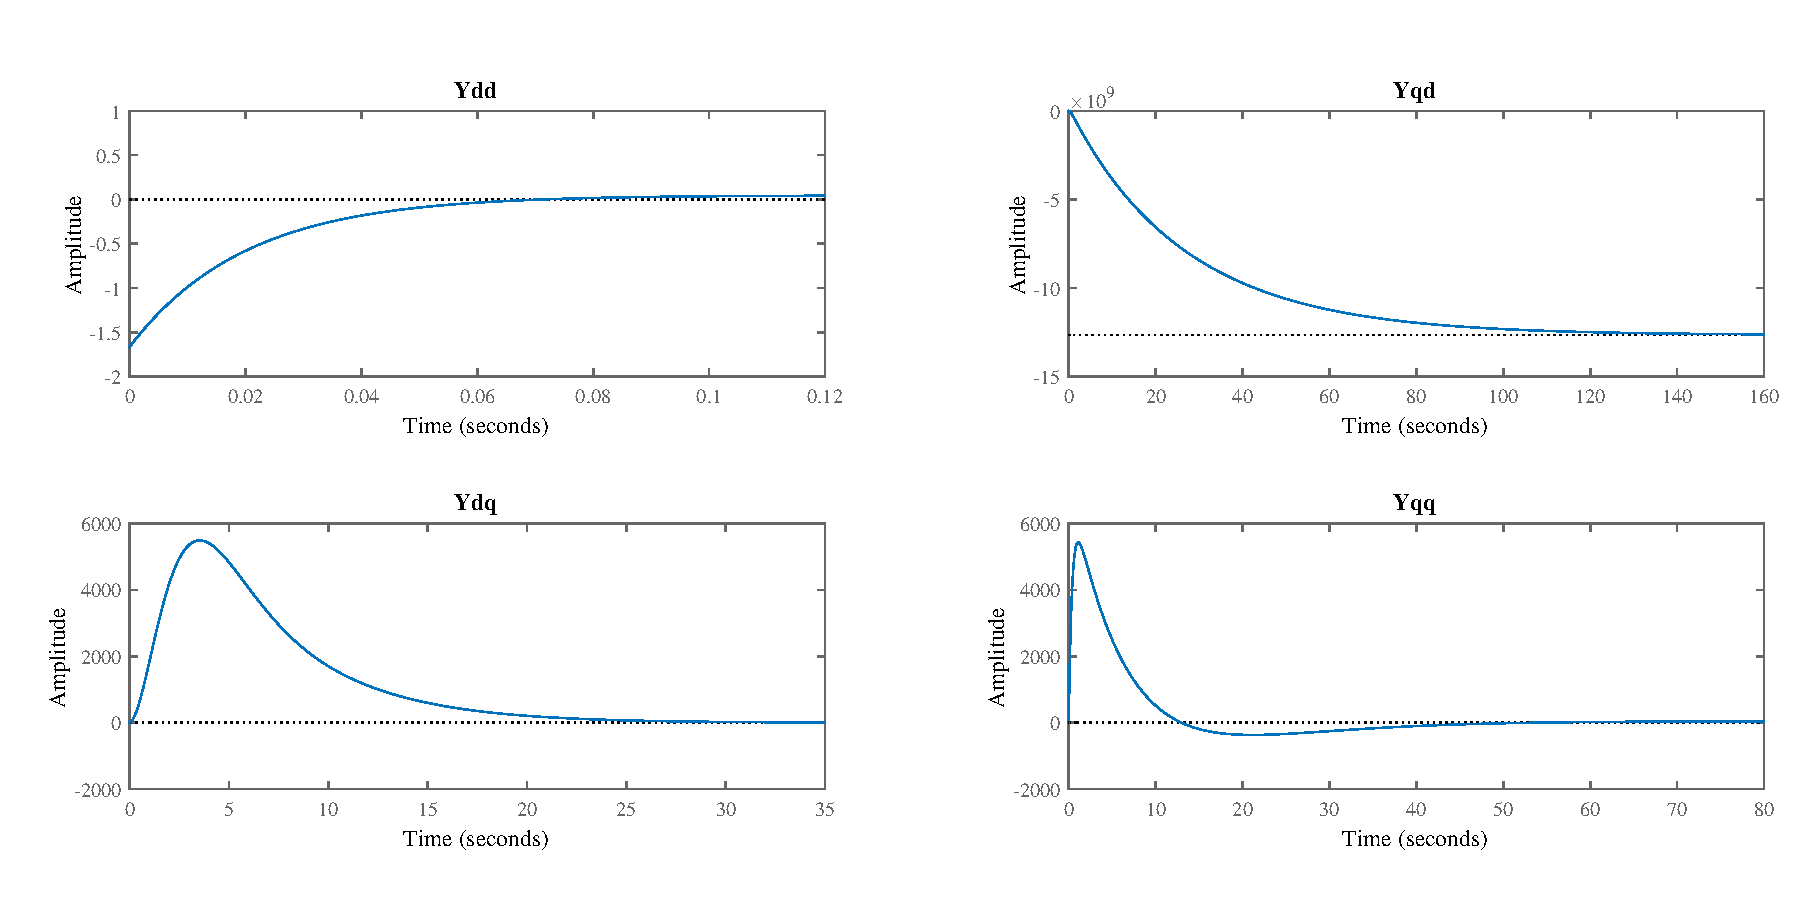
\includegraphics[width=1.2\textwidth]{figures/Base.pdf}}
	\caption[GFL impulse response for $K_I_c=0.1$]{GFL impulse response for $K_I_c=0.1$.}
	\label{res:KIc(0.1)}
	\end{center}
\end{figure}

\begin{figure}[ht]
\begin{center}
    \centering
   \nonindent
   \makebox[]{
	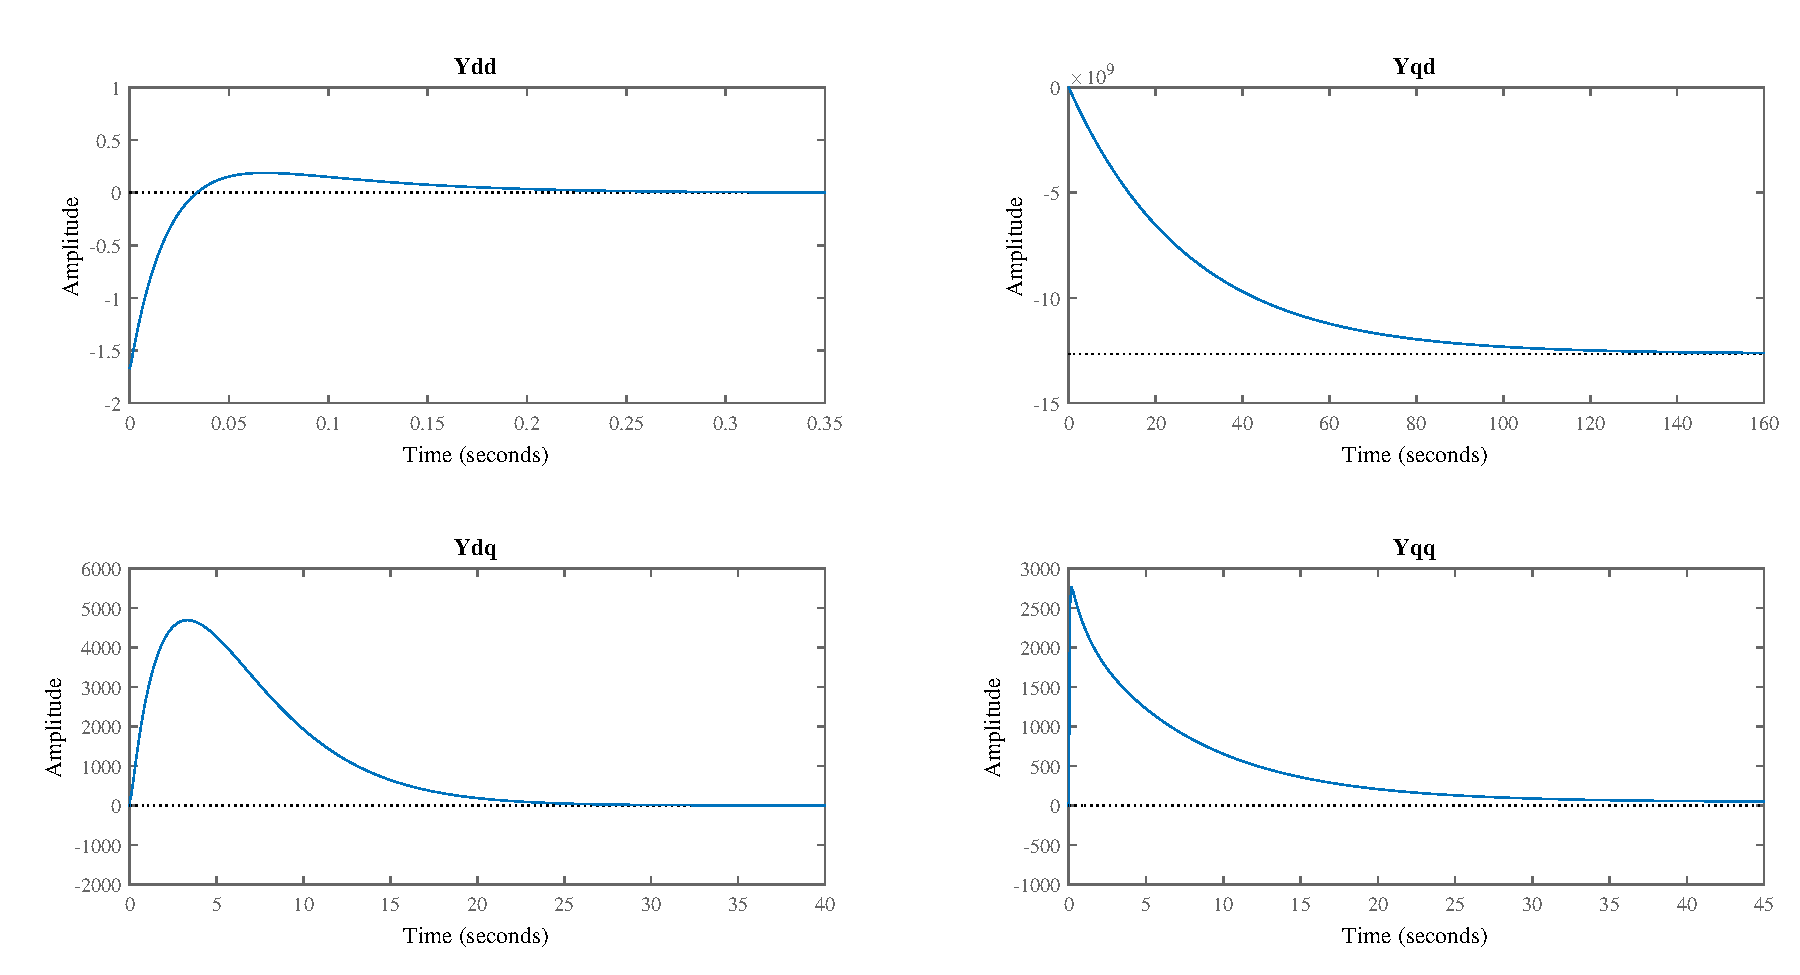
\includegraphics[width=1.2\textwidth]{figures/KIc(10).pdf}}
	\caption[GFL impulse response for $K_I_c=10$]{GFL impulse response for $K_I_c=10$.}
	\label{res:KIc(10)}
	\end{center}
\end{figure}

For analyzing effect of the current loop, amount of the proportional gain ($K_{pc}$) is decreased from 100 to 0.1, as shown in \cref{res:Kpc(10),res:Kpc(0.1),res:Kpc(100)}. Comparing the obtained results  shows that changing $K_{pc}$ to 10 improves the impulse response, by reducing the overshoot of $Y_{qd}$ and $Y_{qq}$. However, The analysis shows that reducing the amount of $K_{pc}$ to 0.01 drives the inverter to unstable margin. So, this amount is fixed to 10. Subsequently, the integral gain ($K_I_c$) of the current control loop is increased from 0.1 to 10, which is illustrated in \cref{res:KIc(0.1),}. Comparing both figures unfolds that this change will decrease the overshoot of $Y_{dq}$ and $Y_{qq}$ from both 6000 to less than 5000 and 3000 P.u respectively. Therefore $K_I_c=10$ is a better selection.

\subsection{Power Control Block}

\begin{figure}[ht]
\begin{center}
    \centering
   \nonindent
   \makebox[]{
	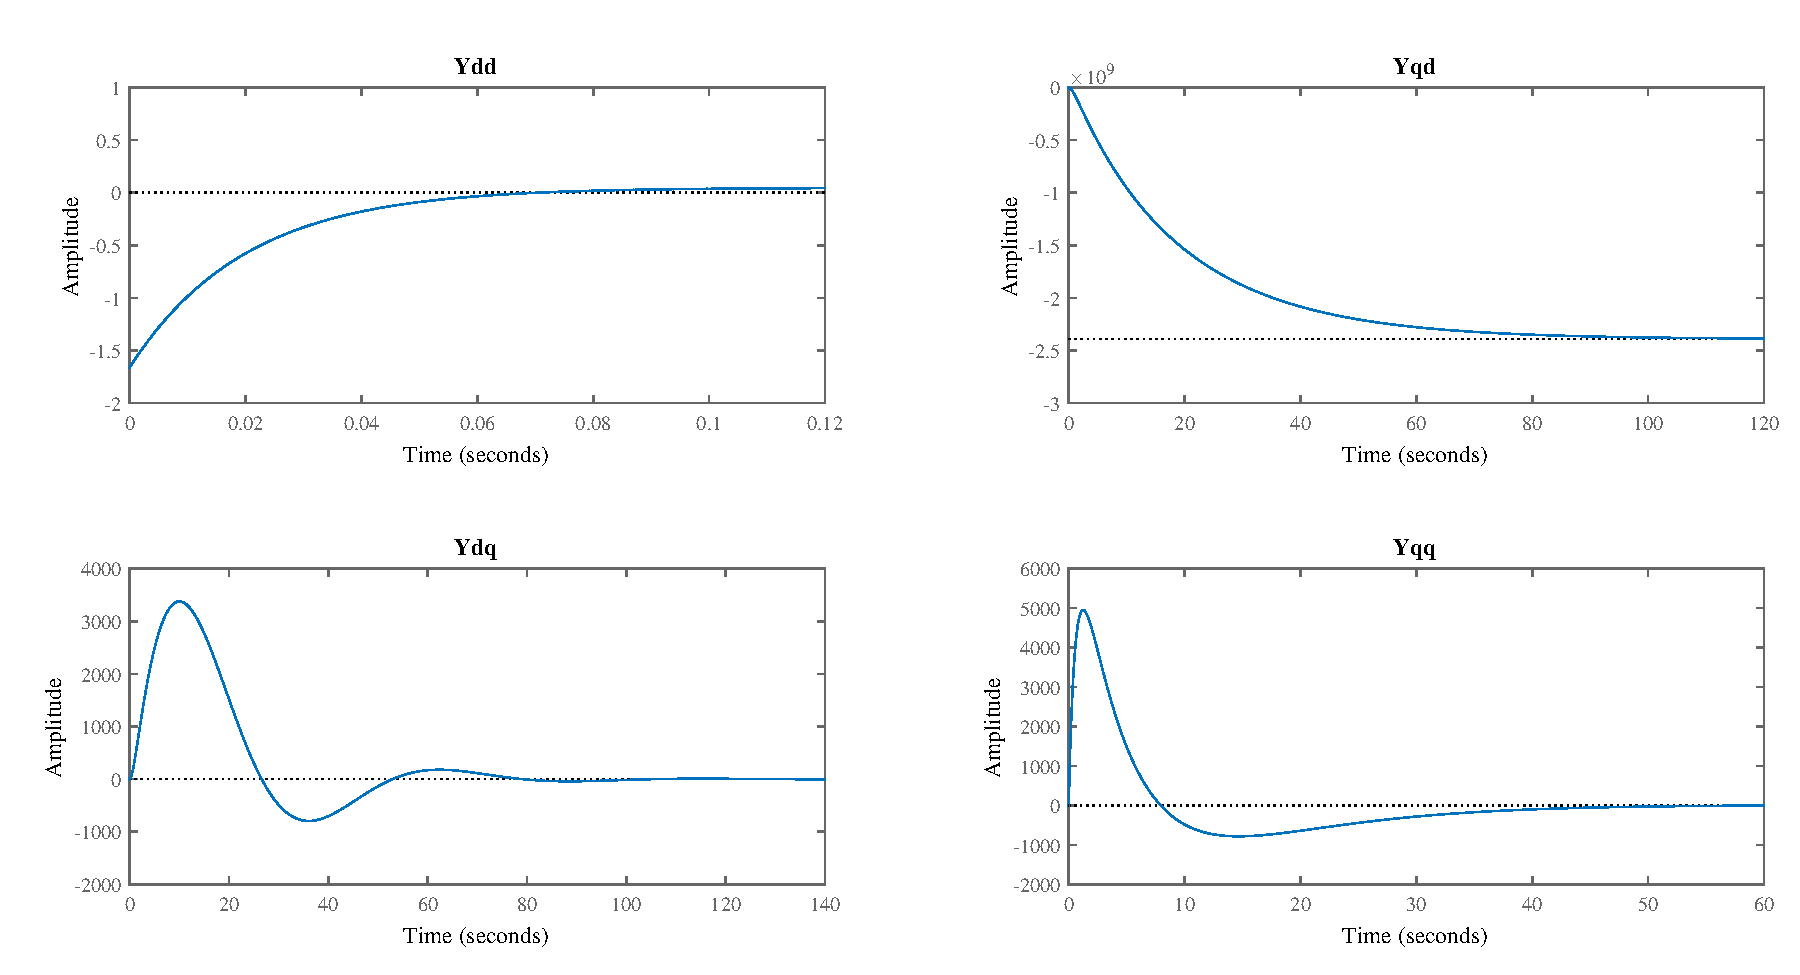
\includegraphics[width=1.2\textwidth]{figures/KpPQ(10).pdf}}
	\caption[GFL impulse response for $K_p_P=10$ and $K_p_Q=10$]{GFL impulse response for $K_p_P=10$ and $K_p_Q=10$.}
	\label{res:Kps(10)}
	\end{center}
\end{figure}

The impact of the proportional gain of active and reactive power ($K_p_P$ and $K_p_Q$) is analyzed by diminishing its amount from 100 to 10, which is depicted in \ref{res:Kps(10)}. The obtained results show that, while the overshoot of $Y_{dq}$ and $Y_{qq}$ is reduced, the dynamic response speed is deteriorated compared to \ref{res:base}.

\begin{figure}[ht]
\begin{center}
    \centering
   \nonindent
   \makebox[]{
	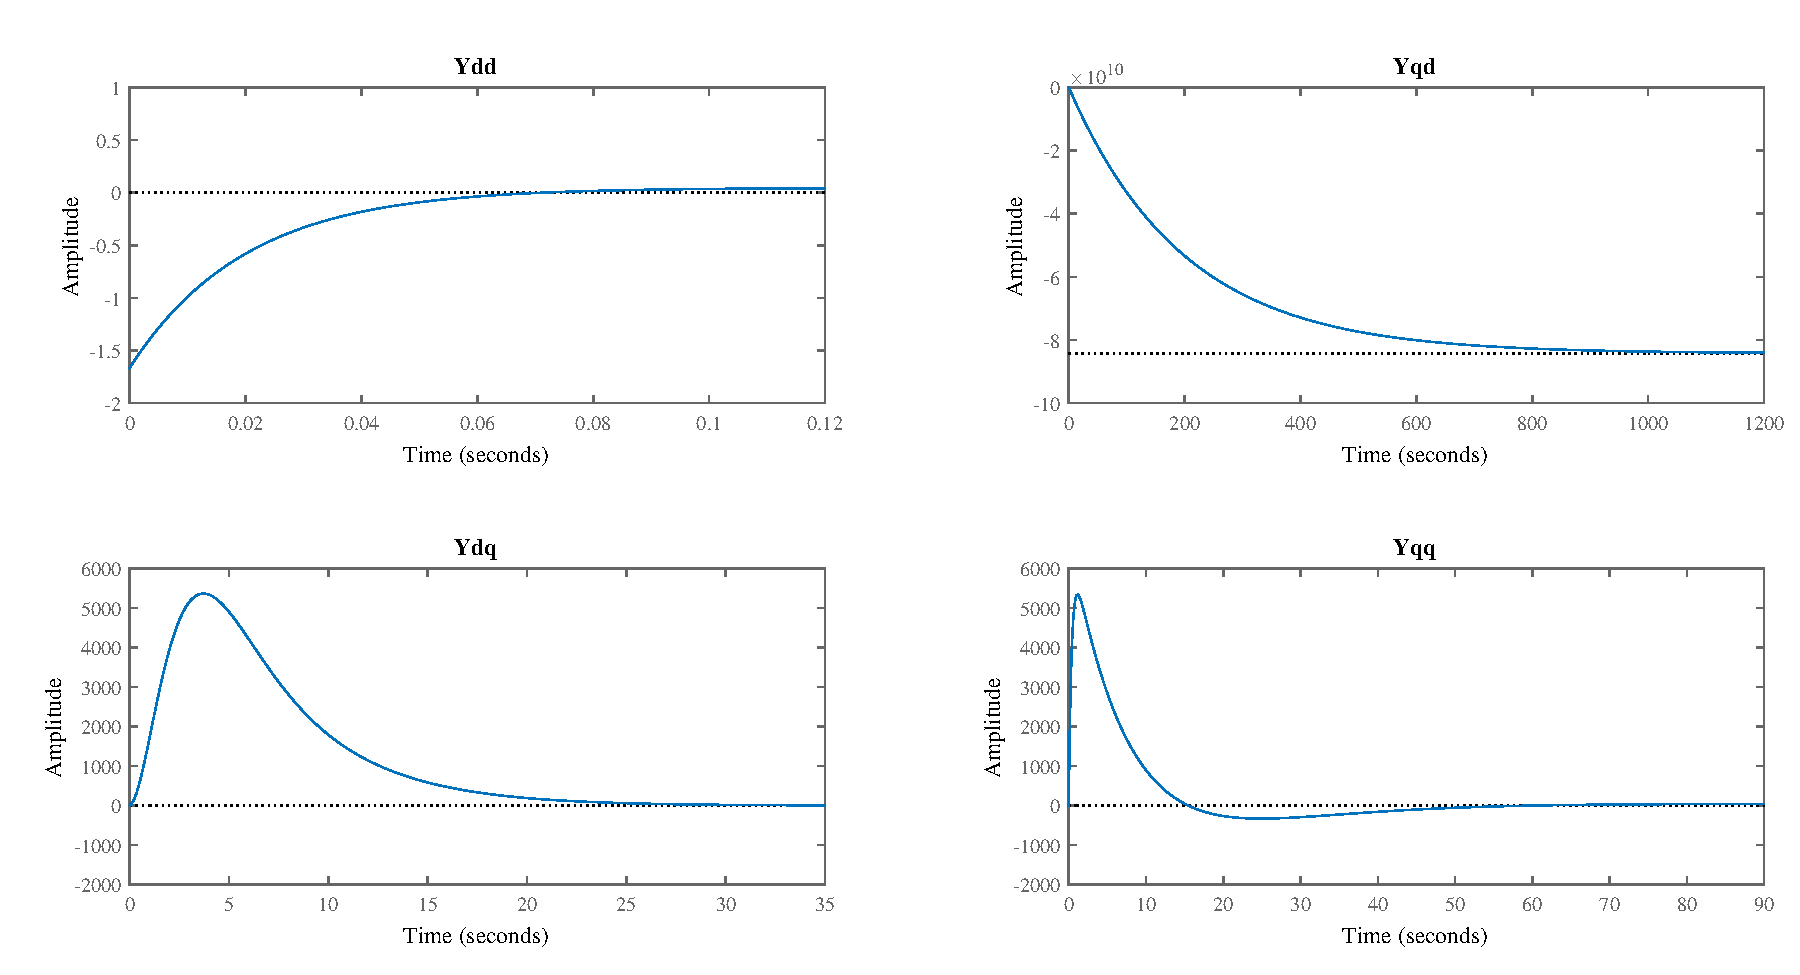
\includegraphics[width=1.2\textwidth]{figures/KiPQ(1).pdf}}
	\caption[GFL impulse response for $K_I_P=1$ and $K_I_Q=1$]{GFL impulse response for $K_I_P=1$ and $K_I_Q=1$}
	\label{res:KIs(1)}
	\end{center}
\end{figure}

Then, the integral gain of active and reactive power ($K_I_P$ and $K_I_Q$) is reduced to 1 from 10. The results are shown in 	\ref{res:KIs(1)}, which has a slower settling time in case of $Y_{qd}$ compared to \ref{res:base}. 

\subsection{\gls{PLL} Block}

\begin{figure}[ht]
\begin{center}
    \centering
   \nonindent
   \makebox[]{
	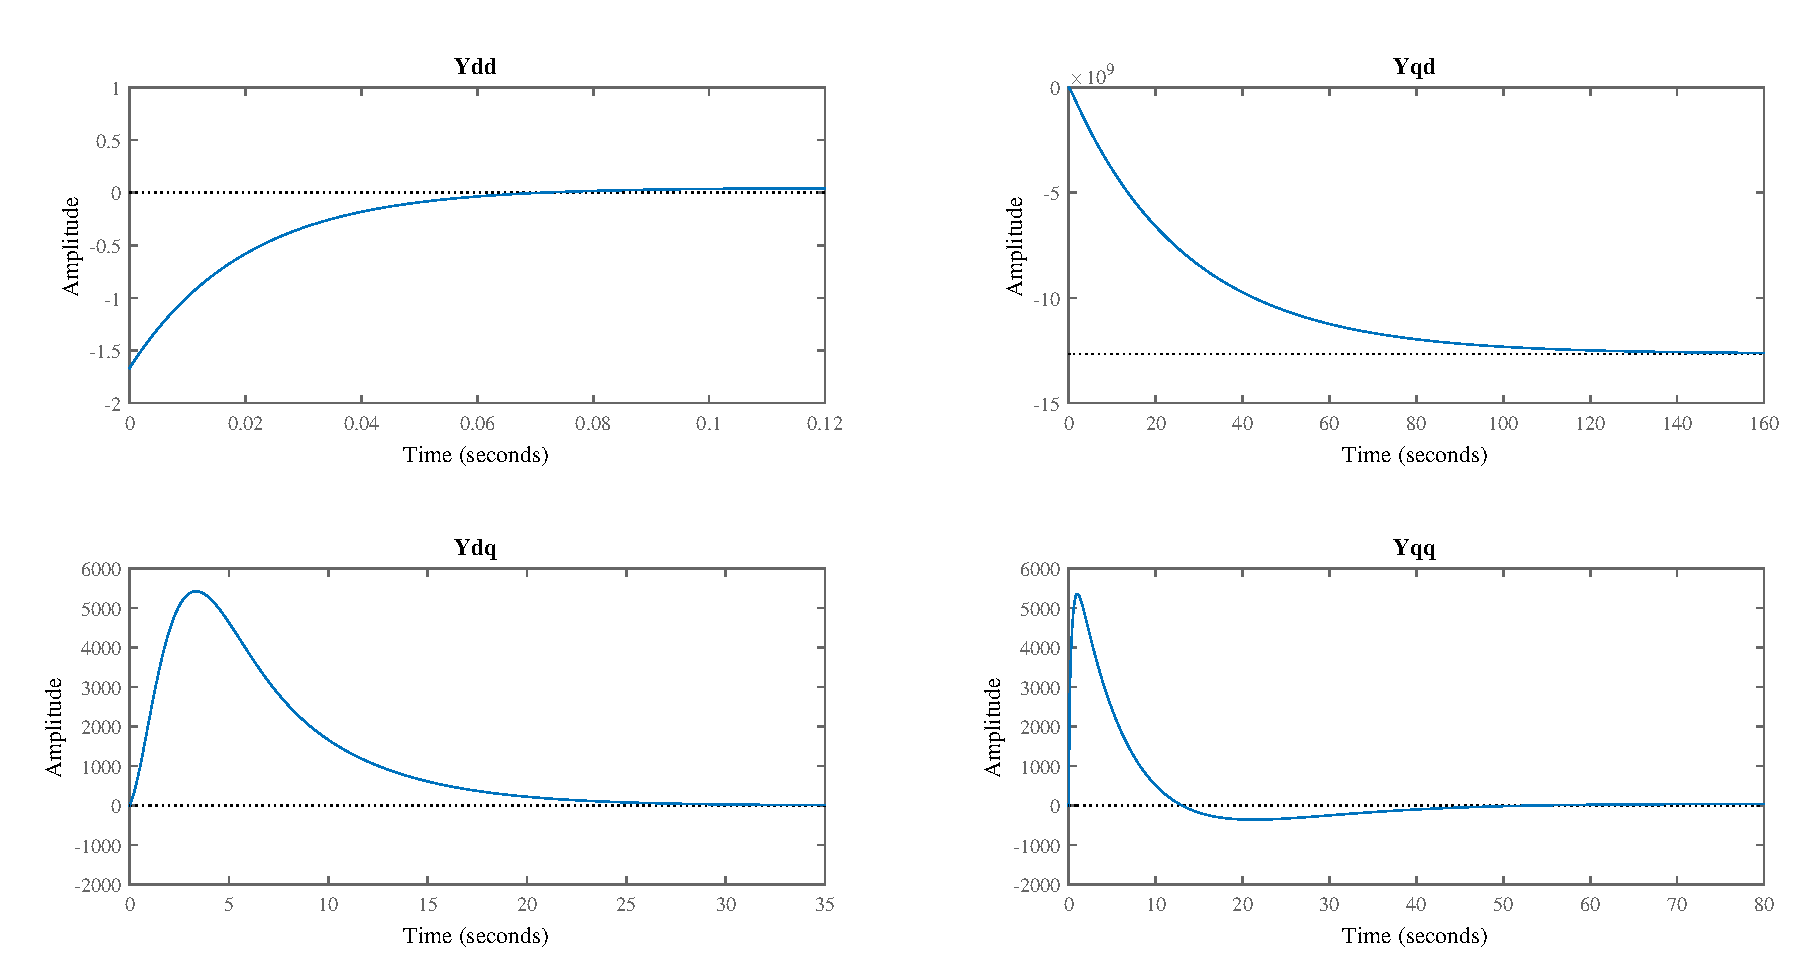
\includegraphics[width=1.2\textwidth]{figures/KpPLL(1000).pdf}}
	\caption[GFL impulse response for $K_P_{PLL}=1000$]{GFL impulse response for $K_P_{PLL}=1000$.}
	\label{res:KPPLL(1000)}
	\end{center}
\end{figure}

The proportional and integral gains of \gls{PLL} block ($K_p_{PLL}$, $K_I_{PLL}$) can have an impact on the small signal stability of the grid-following inverters. First, the effect of the $K_p_{PLL}$ is evaluated by setting its value to 1000, which is shown in \ref{res:KPPLL(1000)}. Comparing \ref{res:KPPLL(1000)} with \ref{res:base} shows that there is no difference between these two results. So, it can be concluded that the amount of $K_p_{PLL}$ is not effective in the case of a GFL inverter.

\begin{figure}[ht]
\begin{center}
    \centering
   \nonindent
   \makebox[]{
	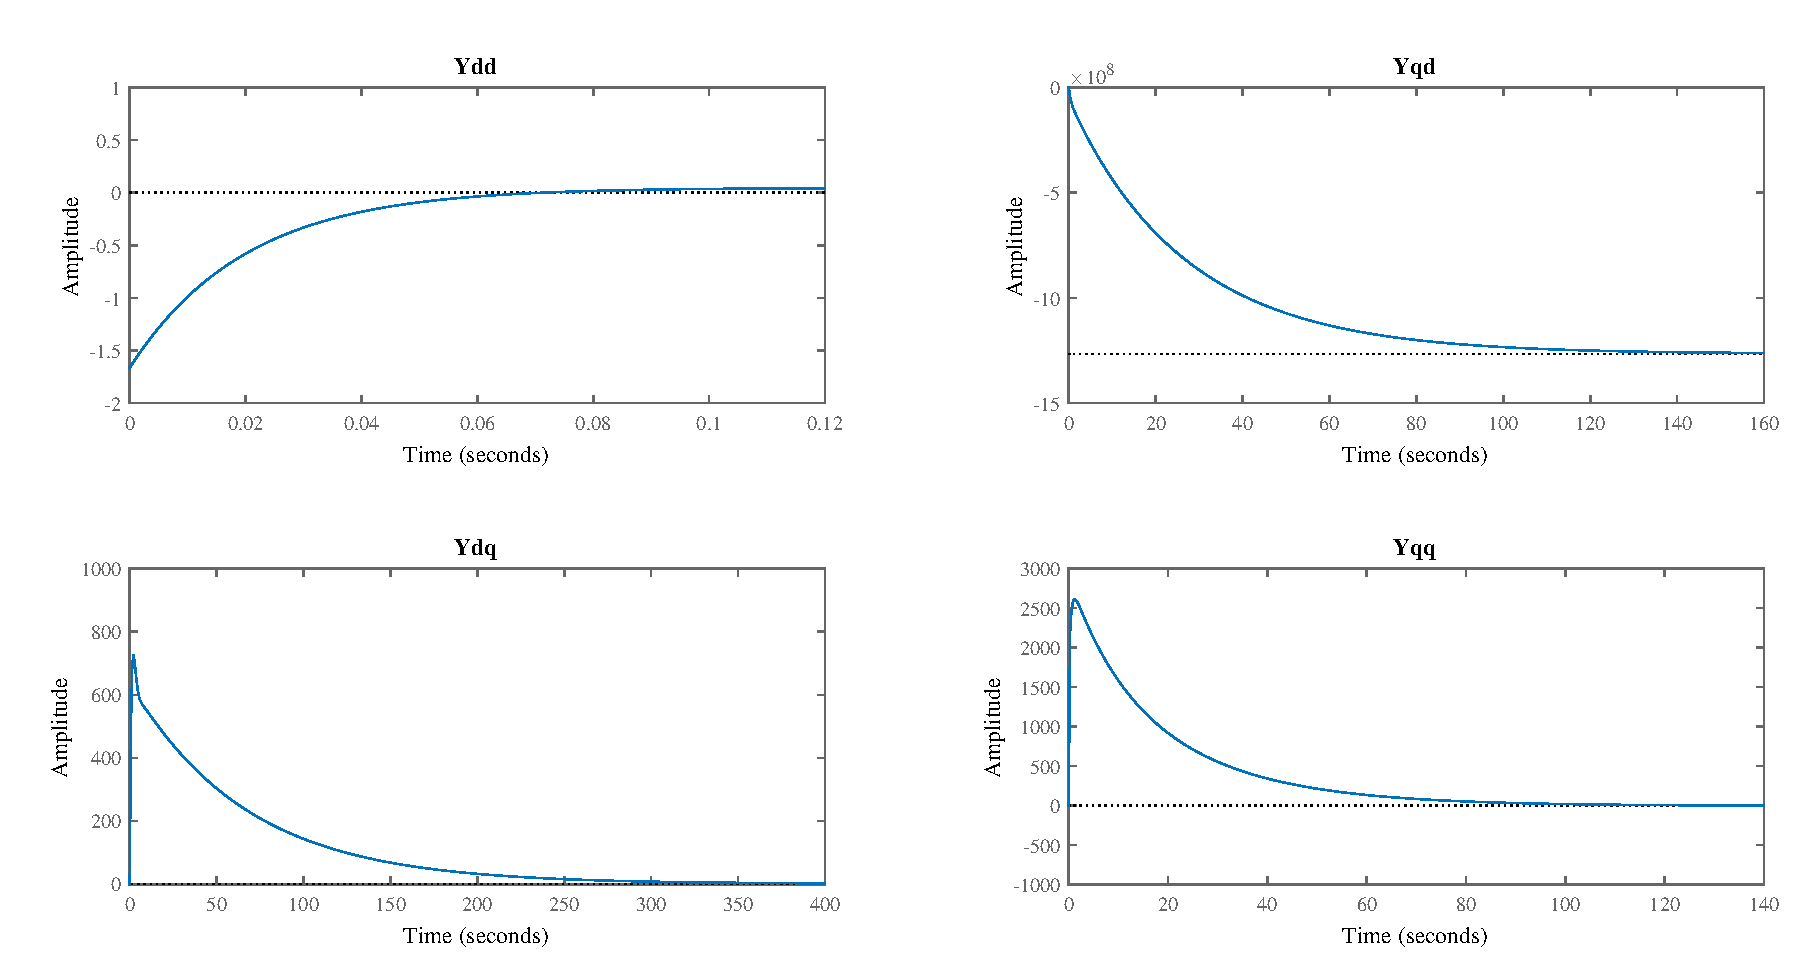
\includegraphics[width=1.2\textwidth]{figures/KiPLL(640).pdf}}
	\caption[GFL impulse response for $K_I_{PLL}=640$]{GFL impulse response for $K_I_{PLL}=640$.}
	\label{res:KIPLL(640)}
	\end{center}
\end{figure}

Secondly, the impact of $K_I_{PLL}$ is measured by setting it to 640. The result is depicted in \ref{res:KIPLL(640)}, and it shows that this change has reduced the overshoot of $Y_{dq}$ and $Y_{qq}$ considerably compared to \ref{res:base}, however the settling time has become slower.

\begin{figure}[ht]
\begin{center}
    \centering
   \nonindent
   \makebox[]{
	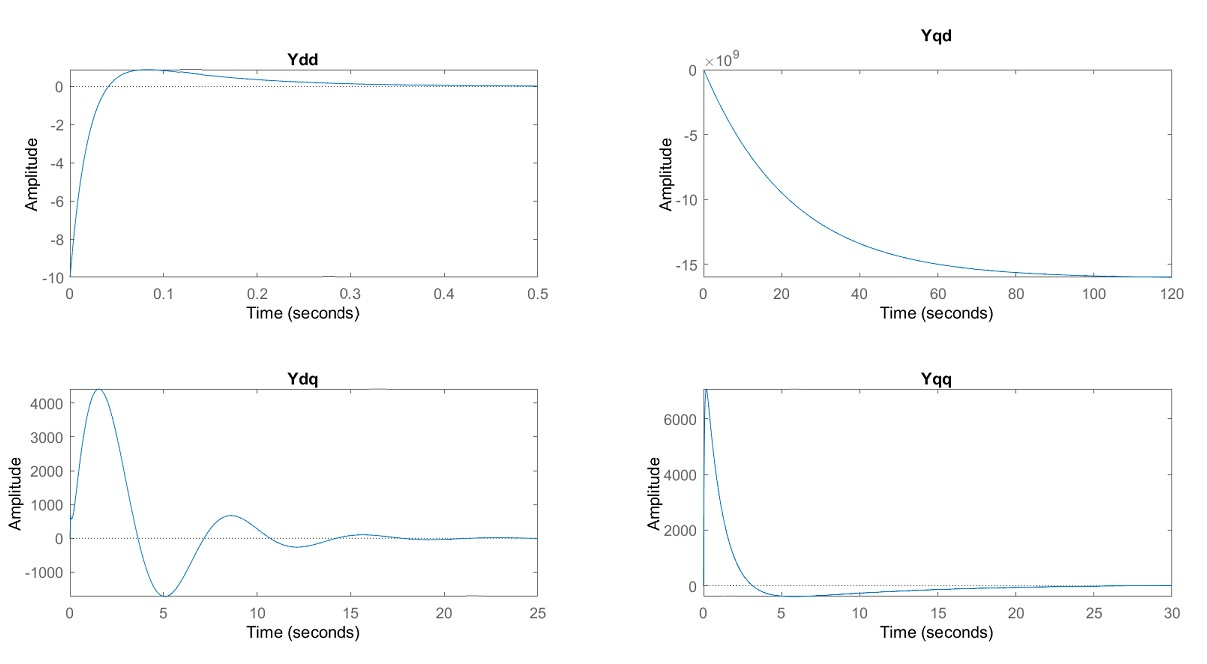
\includegraphics[width=1.2\textwidth]{figures/KIPLL(10000).jpeg}}
	\caption[GFL impulse response for $K_I_{PLL}=10000$]{GFL impulse response for $K_I_{PLL}=10000$.}
	\label{res:KIPLL(10000)}
	\end{center}
\end{figure}

For further analysis, the amount of $K_I_{PLL}$ is set to 10000, which is shown in Figure 11. As it is visible unlike the settling time, the overshoot amount is deteriorated. So, it can be concluded that speed of settling time has direct proportion with the amount of $K_I_{PLL}$, which is inverse in case of overshoot.


\subsection{Output Filter}

\begin{figure}[ht]
\begin{center}
    \centering
   \nonindent
   \makebox[]{
	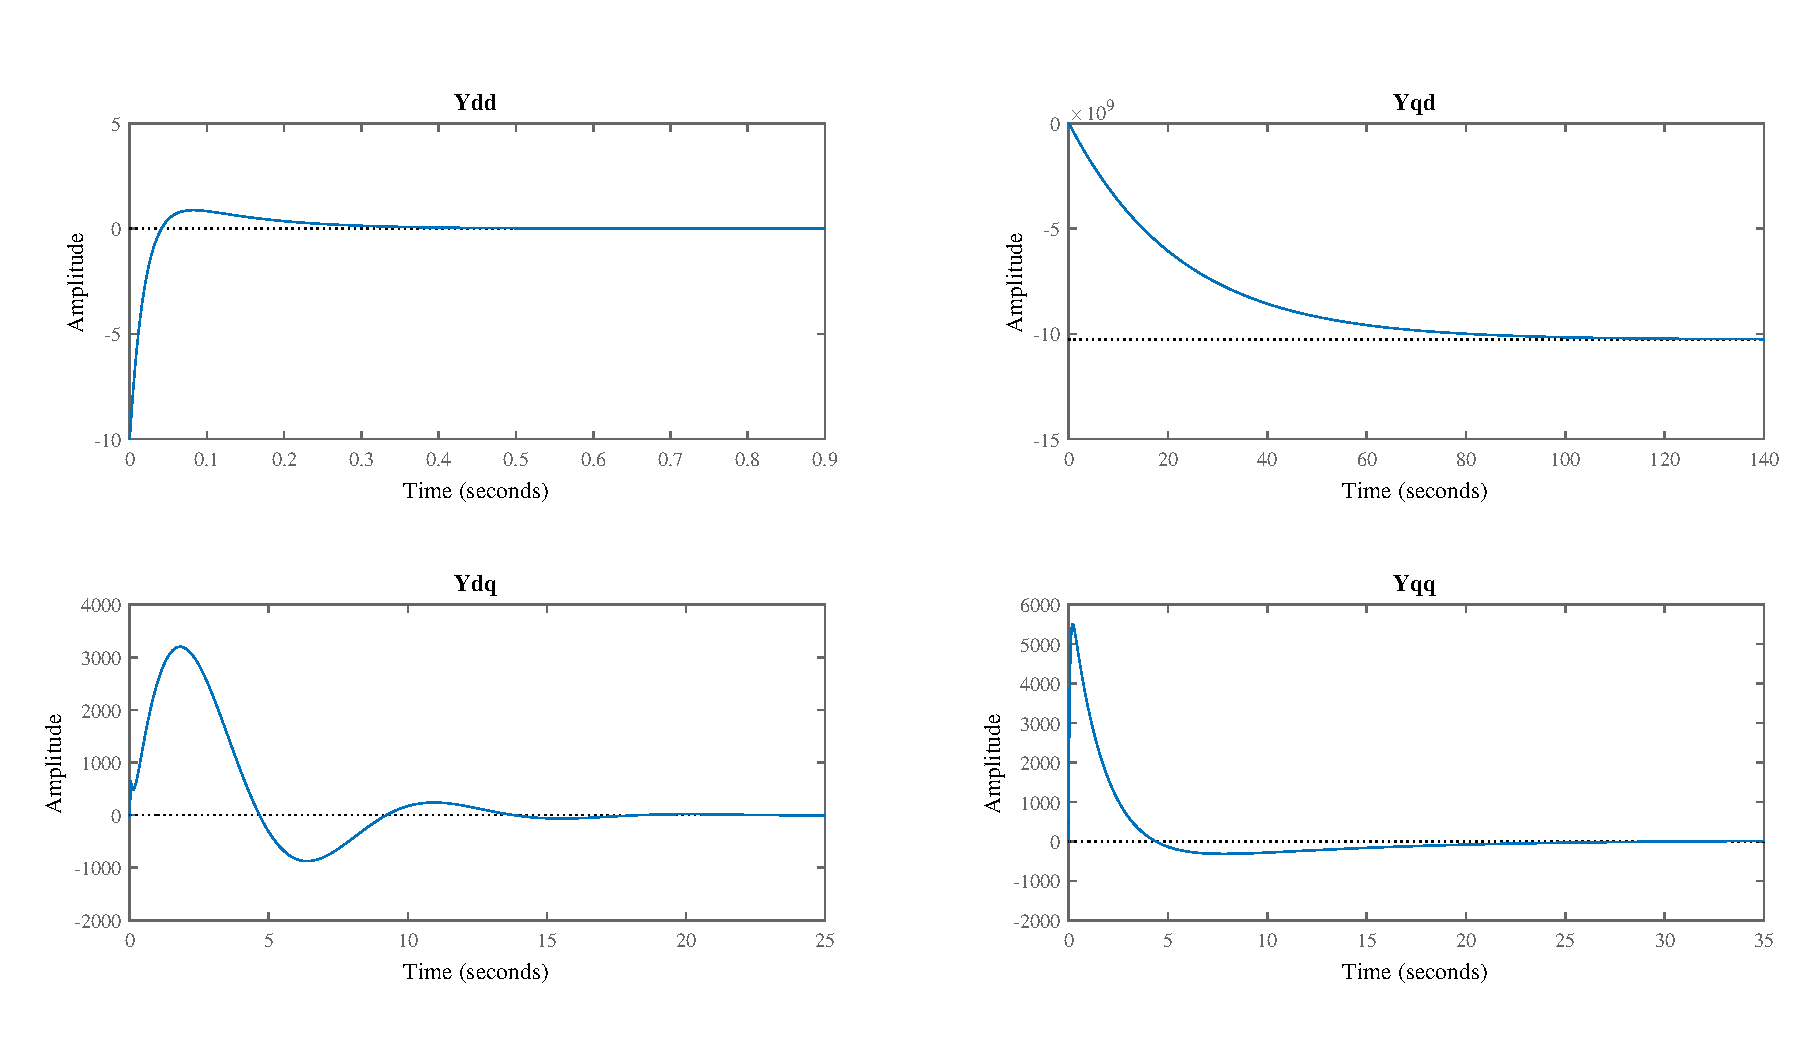
\includegraphics[width=1.2\textwidth]{figures/L1L2(0.1).pdf}}
	\caption[GFL impulse response for $L_1=0.1$ and $L_2=0.1$]{GFL impulse response for $L_1=0.1$ and $L_2=0.1$.}
	\label{res:L1L2(0.1)}
	\end{center}
\end{figure}

\begin{figure}[ht]
\begin{center}
    \centering
   \nonindent
   \makebox[]{
	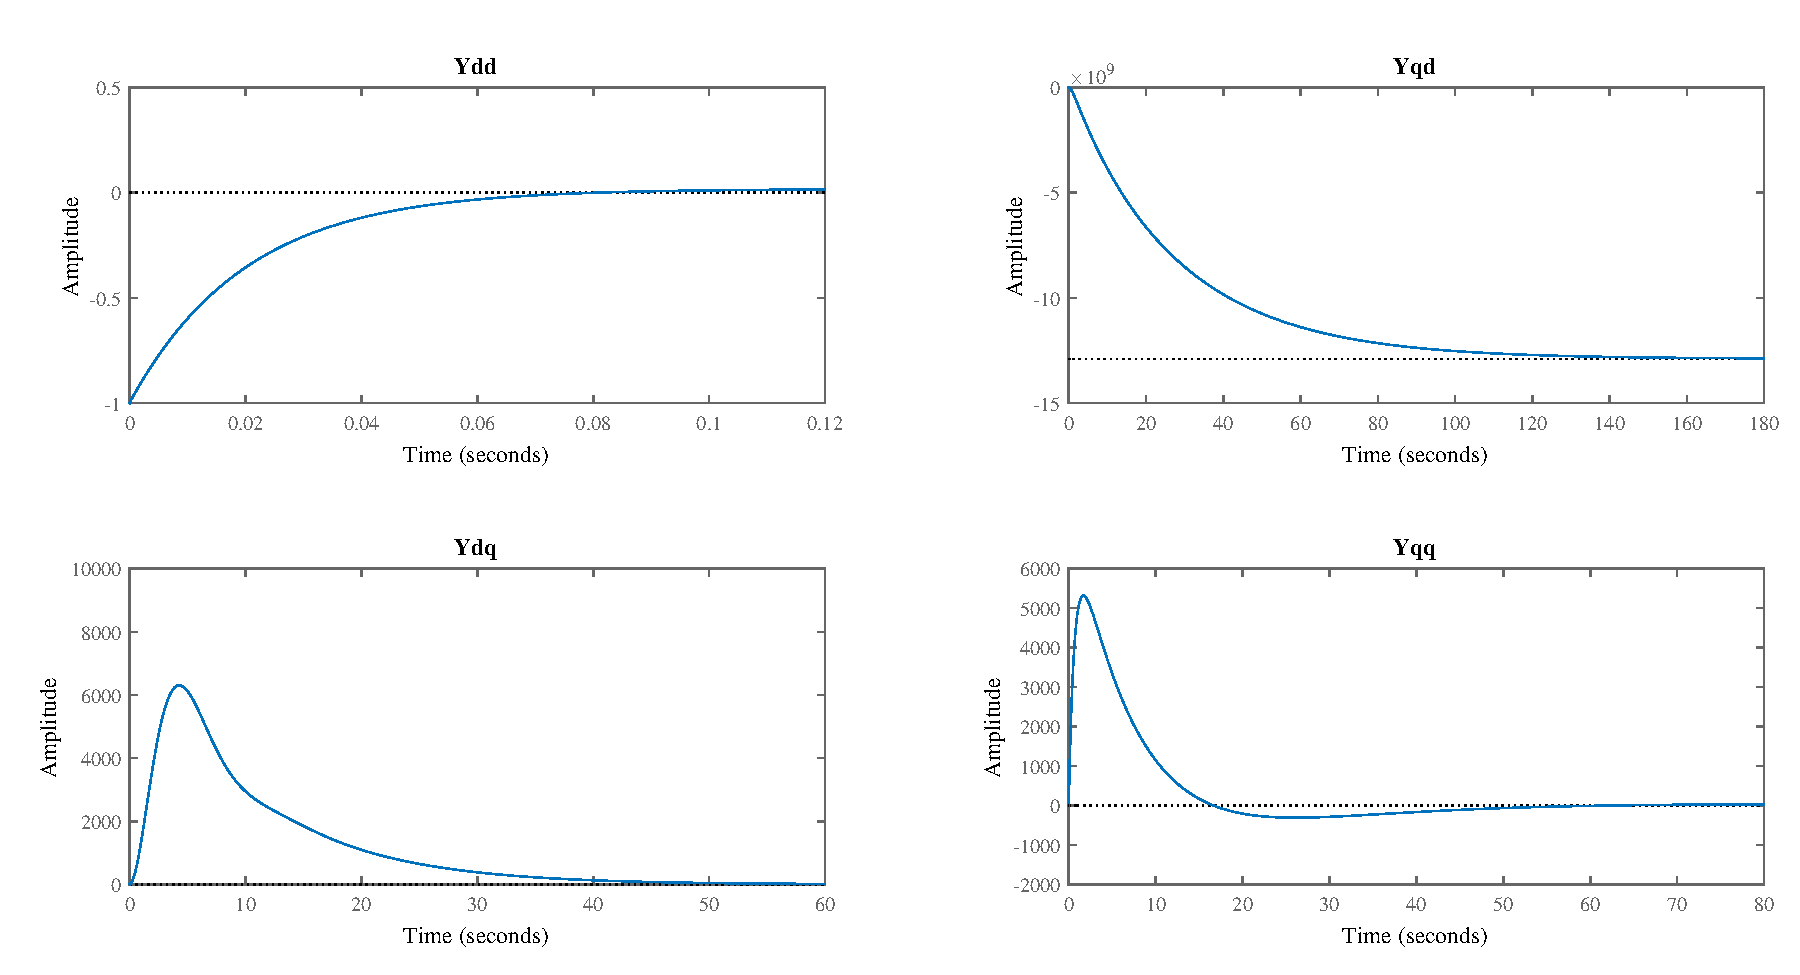
\includegraphics[width=1.2\textwidth]{figures/L1L2(1).pdf}}
	\caption[GFL impulse response for $L_1=1$ and $L_2=1$]{GFL impulse response for $L_1=1$ and $L_2=1$.}
	\label{res:L1L2(1)}
	\end{center}
\end{figure}

 For further analysis, the values of L1 and L2 filters are decreased to 0.1 p.u., and the results are shown in \ref{res:L1L2(0.1)}. Compared to \ref{res:base}, this change only reduced the overshoot amount of $Y_{dq}$. Then, these values are set to 1 p.u. for one more analysis. The results are reported in \ref{res:L1L2(1)}, which only differs from \ref{res:L1L2(0.1)} and \ref{res:base} in terms of the $Y_{dq}$ overshoot.

\begin{figure}[ht]
\begin{center}
    \centering
   \nonindent
   \makebox[]{
	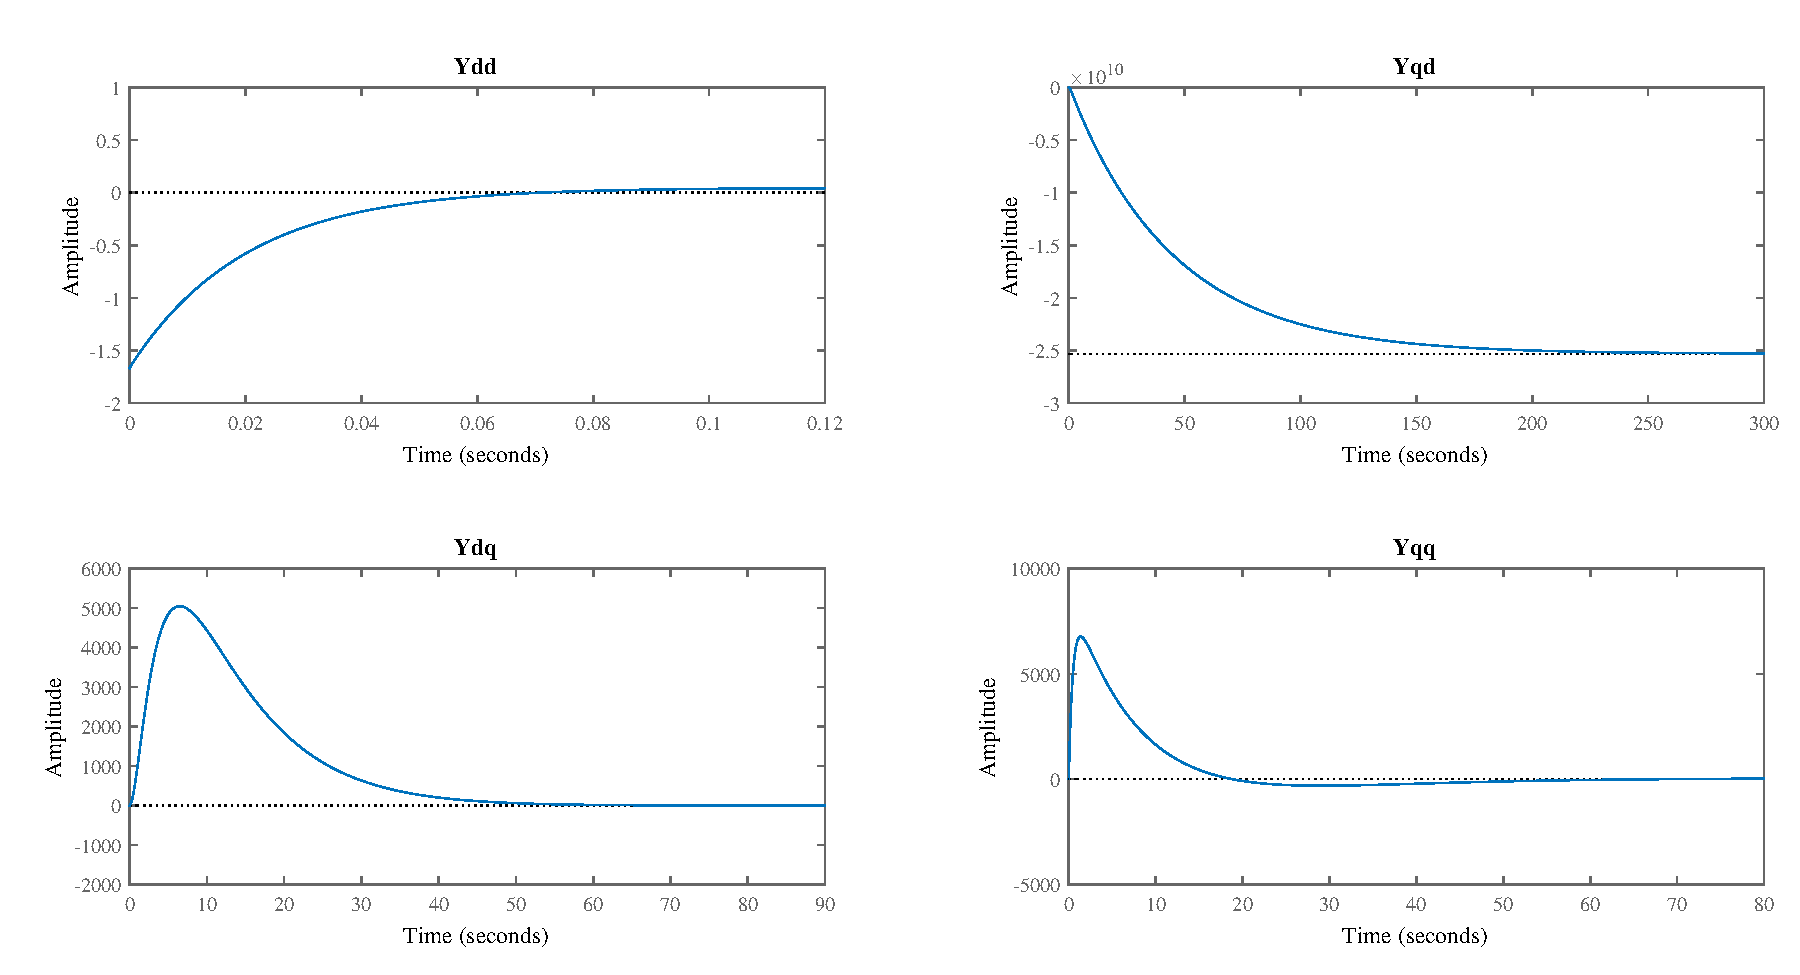
\includegraphics[width=1.2\textwidth]{figures/C(1).pdf}}
	\caption[GFL impulse response for $C=1$]{GFL impulse response for $C=1$.}
	\label{res:C(1)}
	\end{center}
\end{figure}


Finally, the value of the capacitor is changed to 1 p.u. for observing its impact in \ref{res:C(1)}. Evaluating the result did not show any difference. Hence, it can be concluded that the capacitor filter does not affect the response of the inverter, at least in this range.

% text of this chapter goes here
\section{Conclusion}

Among GFMs, the Synchronvertor strategy seemed to be the most complex and challenging to undergo a model reduction. While droop control seemed well behaved, other strategies could not provide stable results with the same parameters. In GFLs, $Y_{dq}$ is observed to be more prone to instability than the other three transfer functions. Also, steady-state angle, $K_I_{PLL}$, and $K_P_{c}$ were observed to be more dominant parameters in system stabilizing. In the same manner, a steady-state angle margin for stability is derived for GFL, which is analogous to internal angle stability in a synchronous generator.
